\documentclass[11pt,a4paper,oneside]{report}
\usepackage[T1]{fontenc}
\usepackage[utf8]{inputenc}
\usepackage{lmodern}
\usepackage[english]{babel}
\usepackage{microtype}
\usepackage{csquotes}
\emergencystretch=2em
\usepackage{geometry}
\geometry{margin=2.7cm}
\usepackage{setspace}
\onehalfspacing
\usepackage{booktabs}
\usepackage{longtable}
\usepackage{array}
\usepackage{graphicx}
\usepackage{xcolor}
\usepackage{tabularx}
\usepackage{tikz}
\usetikzlibrary{arrows.meta,positioning,fit,calc,backgrounds}
\usepackage{listings}
\usepackage{amsmath,amssymb}
\newcommand{\TBD}{\texttt{TBD}}
\usepackage{hyperref}
\usepackage[nameinlink,capitalise]{cleveref}
\lstset{basicstyle=\ttfamily\scriptsize,breaklines=true,columns=fullflexible,keepspaces=true,showstringspaces=false,frame=single}

% Run-7 visual integration. These hooks place the prepared figures/tables at
% the end of the relevant methodological sections without rewriting the frozen
% Run-5/Run-6 prose. The section counter still denotes the section that has just
% finished when the next \section command reaches this hook.
\AddToHook{cmd/section/before}{%
  \ifnum\value{chapter}=5
    \ifnum\value{section}=0 \begin{figure}[htbp]
\centering
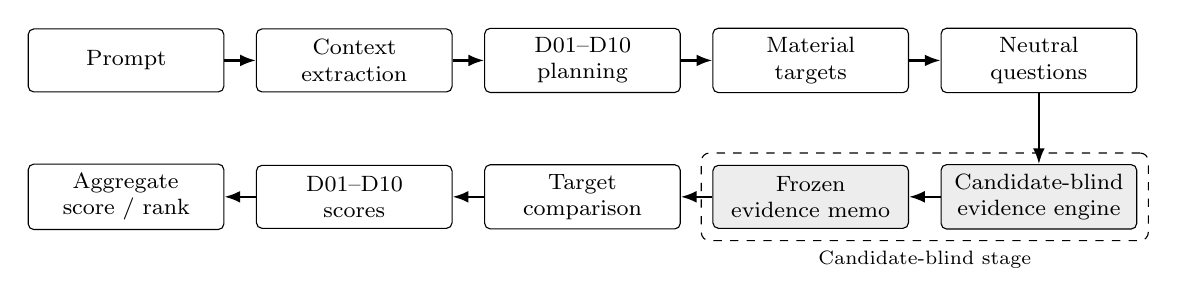
\begin{tikzpicture}[
  node distance=5mm and 4mm,
  box/.style={draw, rounded corners=2pt, align=center, minimum height=8mm, text width=2.25cm, font=\footnotesize},
  blind/.style={box, fill=black!7},
  arrow/.style={-{Latex[length=2mm]}, thick}
]
\node[box] (prompt) {Prompt};
\node[box, right=of prompt] (context) {Context\\extraction};
\node[box, right=of context] (plan) {D01--D10\\planning};
\node[box, right=of plan] (targets) {Material\\targets};
\node[box, right=of targets] (questions) {Neutral\\questions};

\node[blind, below=9mm of questions] (evidence) {Candidate-blind\\evidence engine};
\node[blind, left=of evidence] (memo) {Frozen\\evidence memo};
\node[box, left=of memo] (verdict) {Target\\comparison};
\node[box, left=of verdict] (scores) {D01--D10\\scores};
\node[box, left=of scores] (aggregate) {Aggregate\\score / rank};

\draw[arrow] (prompt) -- (context);
\draw[arrow] (context) -- (plan);
\draw[arrow] (plan) -- (targets);
\draw[arrow] (targets) -- (questions);
\draw[arrow] (questions) -- (evidence);
\draw[arrow] (evidence) -- (memo);
\draw[arrow] (memo) -- (verdict);
\draw[arrow] (verdict) -- (scores);
\draw[arrow] (scores) -- (aggregate);

\node[draw,dashed,rounded corners=3pt,fit=(evidence)(memo),inner sep=4pt,label={[font=\scriptsize]below:Candidate-blind stage}] {};
\end{tikzpicture}
\caption{Architecture of the standalone evidence-grounded cultural verifier. The shaded stage is structurally separated from candidate and target objects after verification-question generation.}
\label{fig:verifier-architecture}
\end{figure}
\fi
    \ifnum\value{section}=7 \begin{figure}[htbp]
\centering
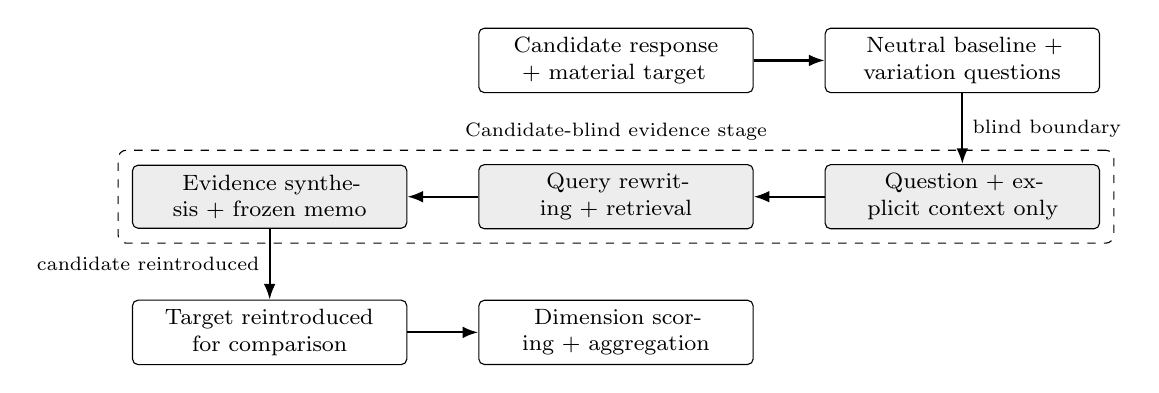
\begin{tikzpicture}[
  node distance=5mm,
  box/.style={draw, rounded corners=2pt, align=center, minimum height=8mm, text width=3.25cm, font=\footnotesize},
  blind/.style={box, fill=black!7},
  arrow/.style={-{Latex[length=2mm]}, thick}
]
\node[box] (candidate) {Candidate response + material target};
\node[box, right=9mm of candidate] (questions) {Neutral baseline + variation questions};
\draw[arrow] (candidate) -- (questions);

\node[blind, below=9mm of questions] (query) {Question + explicit context only};
\node[blind, left=9mm of query] (retrieve) {Query rewriting + retrieval};
\node[blind, left=9mm of retrieve] (memo) {Evidence synthesis + frozen memo};
\draw[arrow] (questions) -- node[right,font=\scriptsize]{blind boundary} (query);
\draw[arrow] (query) -- (retrieve);
\draw[arrow] (retrieve) -- (memo);

\node[box, below=9mm of memo] (compare) {Target reintroduced for comparison};
\node[box, right=9mm of compare] (score) {Dimension scoring + aggregation};
\draw[arrow] (memo) -- node[left,font=\scriptsize]{candidate reintroduced} (compare);
\draw[arrow] (compare) -- (score);

\node[draw,dashed,rounded corners=3pt,fit=(query)(retrieve)(memo),inner sep=5pt,label={[font=\scriptsize]above:Candidate-blind evidence stage}] {};
\end{tikzpicture}
\caption{Location of the candidate-blind boundary. Blindness begins only after target-derived verification questions have been generated; question wording can therefore still transmit framing.}
\label{fig:blind-boundary}
\end{figure}
\fi
    \ifnum\value{section}=10 \begin{table}[htbp]
\centering
\footnotesize
\setlength{\tabcolsep}{4pt}
\renewcommand{\arraystretch}{1.08}
\caption{Source classes used by the evidence stage. Classification is categorical and does not constitute a universal quality score.}
\label{tab:source-types}
\begin{tabularx}{\textwidth}{p{3.5cm}X}
\toprule
\textbf{Runtime label} & \textbf{Intended provenance class} \\
\midrule
\nolinkurl{official_legal} & Official legal, regulatory, governmental or other authoritative primary source \\
\nolinkurl{academic_peer_reviewed} & Peer-reviewed scholarly publication \\
\nolinkurl{statistical_survey} & Statistical, polling or survey evidence \\
\nolinkurl{institutional_professional} & Institutional or professional guidance that is not itself binding law \\
\nolinkurl{community_insider} & Community or insider account relevant to lived practice \\
\nolinkurl{general_explanatory} & General explanatory source without stronger provenance \\
\nolinkurl{commercial_lifestyle} & Commercial or lifestyle-oriented source \\
\nolinkurl{unknown} & Provenance cannot be classified reliably from the available material \\
\bottomrule
\end{tabularx}
\end{table}
\fi
    \ifnum\value{section}=17 \begin{figure}[htbp]
\centering
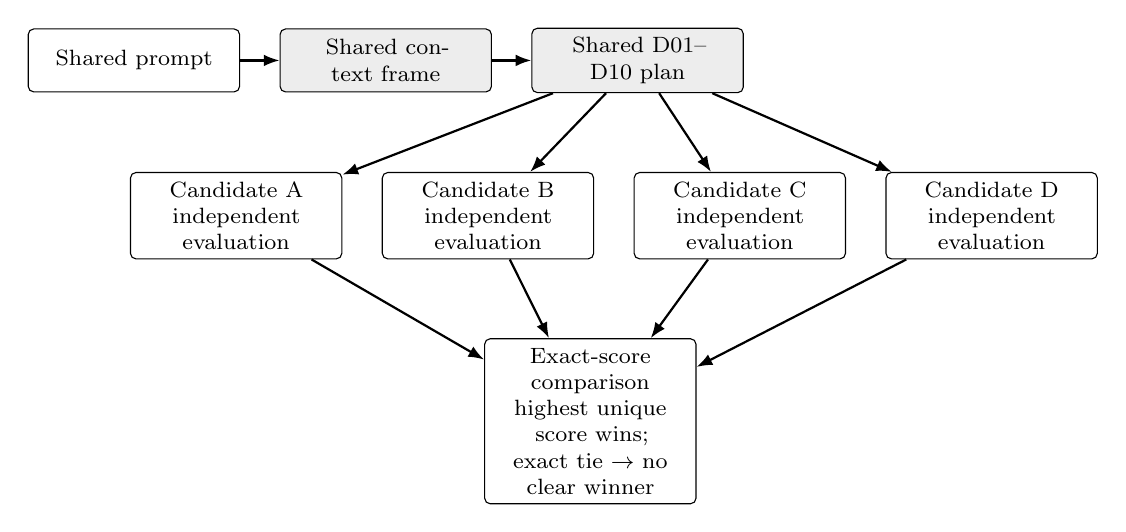
\begin{tikzpicture}[
  node distance=5mm and 5mm,
  box/.style={draw, rounded corners=2pt, align=center, minimum height=8mm, text width=2.45cm, font=\footnotesize},
  shared/.style={box, fill=black!7},
  arrow/.style={-{Latex[length=2mm]}, thick}
]
\node[box] (prompt) {Shared prompt};
\node[shared, right=of prompt] (context) {Shared context frame};
\node[shared, right=of context] (plan) {Shared D01--D10 plan};
\draw[arrow] (prompt) -- (context);
\draw[arrow] (context) -- (plan);

\node[box, below left=10mm and 24mm of plan] (a) {Candidate A\\independent evaluation};
\node[box, right=of a] (b) {Candidate B\\independent evaluation};
\node[box, right=of b] (c) {Candidate C\\independent evaluation};
\node[box, right=of c] (d) {Candidate D\\independent evaluation};
\foreach \x in {a,b,c,d} {\draw[arrow] (plan) -- (\x);}

\node[box, below=10mm of b, xshift=13mm] (rank) {Exact-score comparison\\highest unique score wins; exact tie $\rightarrow$ no clear winner};
\foreach \x in {a,b,c,d} {\draw[arrow] (\x) -- (rank);}
\end{tikzpicture}
\caption{Best-of-4 evaluation with shared prompt-level planning and independent candidate evaluation. Primary/secondary dimension roles do not change score weights.}
\label{fig:best-of4}
\end{figure}
\fi
    \ifnum\value{section}=18 \begin{figure}[htbp]
\centering
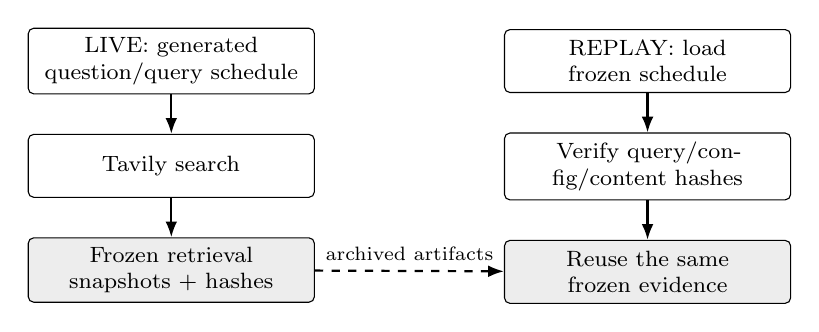
\begin{tikzpicture}[
  node distance=5mm and 10mm,
  box/.style={draw, rounded corners=2pt, align=center, minimum height=8mm, text width=3.4cm, font=\footnotesize},
  artifact/.style={box, fill=black!7},
  arrow/.style={-{Latex[length=2mm]}, thick}
]
\node[box] (liveq) {LIVE: generated question/query schedule};
\node[box, below=of liveq] (search) {Tavily search};
\node[artifact, below=of search] (snap) {Frozen retrieval snapshots + hashes};

\node[box, right=24mm of liveq] (replayq) {REPLAY: load frozen schedule};
\node[box, below=of replayq] (verify) {Verify query/config/content hashes};
\node[artifact, below=of verify] (reuse) {Reuse the same frozen evidence};

\draw[arrow] (liveq) -- (search);
\draw[arrow] (search) -- (snap);
\draw[arrow] (replayq) -- (verify);
\draw[arrow] (verify) -- (reuse);
\draw[arrow,dashed] (snap) -- node[above,font=\scriptsize]{archived artifacts} (reuse);
\end{tikzpicture}
\caption{LIVE and REPLAY evidence modes. REPLAY fixes the retrieval artifacts and has no live-search fallback, but semantic model stages still execute and are therefore not guaranteed to be bitwise deterministic.}
\label{fig:live-replay}
\end{figure}
\fi
  \fi
  \ifnum\value{chapter}=6
    \ifnum\value{section}=1 \begin{figure}[htbp]
\centering
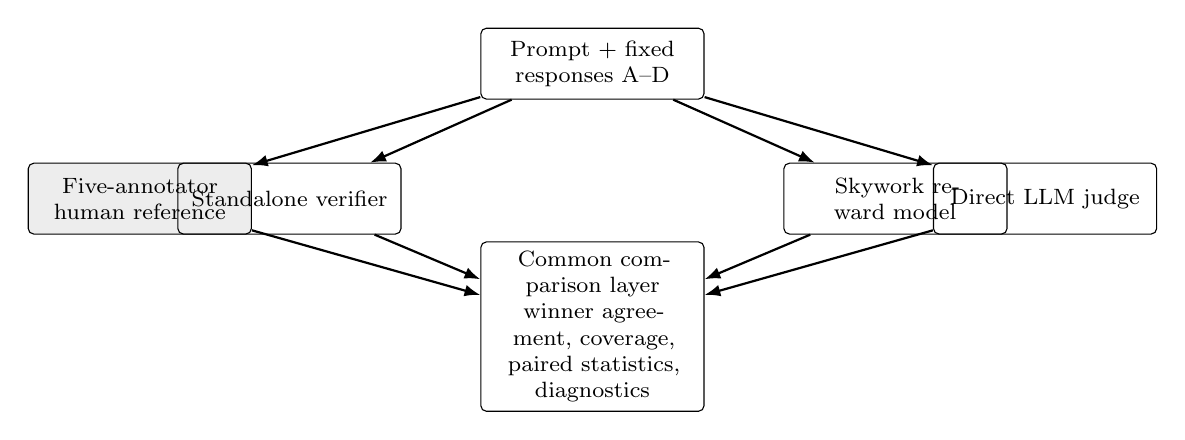
\begin{tikzpicture}[
  node distance=6mm and 5mm,
  box/.style={draw, rounded corners=2pt, align=center, minimum height=9mm, text width=2.6cm, font=\footnotesize},
  ref/.style={box, fill=black!7},
  arrow/.style={-{Latex[length=2mm]}, thick}
]
\node[box] (item) {Prompt + fixed responses A--D};
\node[ref, below left=8mm and 29mm of item] (human) {Five-annotator human reference};
\node[box, below left=8mm and 10mm of item] (verifier) {Standalone verifier};
\node[box, below right=8mm and 10mm of item] (rm) {Skywork reward model};
\node[box, below right=8mm and 29mm of item] (judge) {Direct LLM judge};
\foreach \x in {human,verifier,rm,judge} {\draw[arrow] (item) -- (\x);}
\node[box, below=18mm of item] (compare) {Common comparison layer\\winner agreement, coverage, paired statistics, diagnostics};
\foreach \x in {human,verifier,rm,judge} {\draw[arrow] (\x) -- (compare);}
\end{tikzpicture}
\caption{Overall empirical design. The human reference and three automated systems operate independently on the same fixed Best-of-4 items before comparative analysis.}
\label{fig:research-design}
\end{figure}
\begin{table}[htbp]
\centering
\footnotesize
\setlength{\tabcolsep}{3pt}
\renewcommand{\arraystretch}{1.08}
\caption{Independent systems in the primary comparative evaluation.}
\label{tab:evaluation-systems}
\begin{tabularx}{\textwidth}{p{3.0cm}p{2.6cm}p{2.5cm}X}
\toprule
\textbf{System} & \textbf{Input} & \textbf{Primary output} & \textbf{Information deliberately unavailable} \\
\midrule
Human reference & Prompt + A--D & Categorical vote + confidence & Verifier, RM and direct-judge outputs; provisional labels \\
Standalone verifier & Prompt + one response at a time & D01--D10 scores, evidence trace, overall score/rank & Human labels, RM outputs, benchmark answers, expected issues \\
Skywork RM & Prompt + one response & Raw reward and induced winner & D01--D10, retrieval evidence, human labels, verifier outputs \\
Direct LLM judge & Prompt + A--D & A/B/C/D/no-clear-winner choice & Retrieval evidence, RM scores, human labels, verifier outputs \\
\bottomrule
\end{tabularx}
\end{table}
\fi
    \ifnum\value{section}=4 \begin{figure}[htbp]
\centering
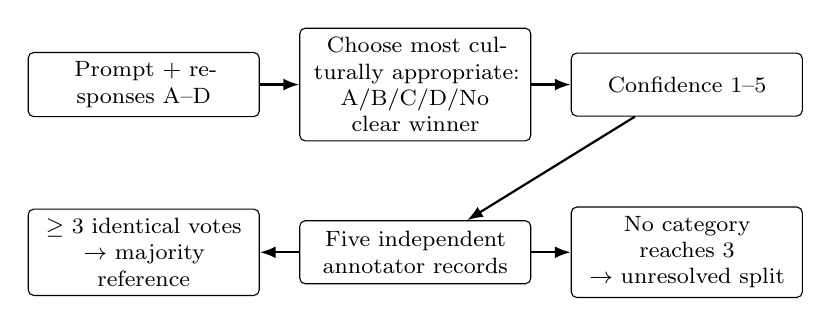
\begin{tikzpicture}[
  node distance=6mm and 5mm,
  box/.style={draw, rounded corners=2pt, align=center, minimum height=8mm, text width=2.7cm, font=\footnotesize},
  arrow/.style={-{Latex[length=2mm]}, thick}
]
\node[box] (item) {Prompt + responses A--D};
\node[box, right=of item] (task) {Choose most culturally appropriate: A/B/C/D/No clear winner};
\node[box, right=of task] (conf) {Confidence 1--5};
\draw[arrow] (item) -- (task);
\draw[arrow] (task) -- (conf);

\node[box, below=10mm of task] (five) {Five independent annotator records};
\node[box, left=of five] (majority) {$\geq 3$ identical votes\\$\rightarrow$ majority reference};
\node[box, right=of five] (split) {No category reaches 3\\$\rightarrow$ unresolved split};
\draw[arrow] (conf) -- (five);
\draw[arrow] (five) -- (majority);
\draw[arrow] (five) -- (split);
\end{tikzpicture}
\caption{Human annotation and reference-construction protocol. Confidence is retained as a secondary measure and does not weight the primary categorical vote.}
\label{fig:human-annotation}
\end{figure}
\fi
    \ifnum\value{section}=5 \begin{table}[htbp]
\centering
\footnotesize
\setlength{\tabcolsep}{4pt}
\renewcommand{\arraystretch}{1.08}
\caption{Experimental configuration: implemented constants and values that remain to be frozen before the final run.}
\label{tab:experiment-freeze}
\begin{tabularx}{\textwidth}{p{4.2cm}X}
\toprule
\textbf{Field} & \textbf{Frozen/current value} \\
\midrule
Verifier architecture & \texttt{cultverify-1.0.0}; implementation commit \texttt{2e546a48ba0950e78f7bd244b5b37b7b475ccf2d} \\
Semantic model/provider/revision & \texttt{[FINAL VERIFIER MODEL / PROVIDER / REVISION TO BE FROZEN]} \\
Temperature & 0 in current configuration; confirm in final manifest \\
Target budget & Maximum 3 material targets \\
Retrieval depth & \texttt{top\_k}=3 accepted documents per query; maximum 2 retrieval rounds \\
Evidence mode & LIVE acquisition followed by primary REPLAY evaluation \\
Reward-model baseline & \texttt{Skywork/Skywork-Reward-V2-Qwen3-4B}; exact-top tie must map to \texttt{no\_clear\_winner} \\
Direct judge & \texttt{[MODEL / PROMPT / ORDER SCHEDULE / SEED TO BE FROZEN]} \\
Evaluation sample & PLT001--PLT030 fixed evaluation set unless a confirmatory unseen set is added before freeze \\
Human annotations & Five annotators planned; final export/hash pending \\
Statistical seed & \texttt{[TO BE FROZEN BEFORE RESULTS]} \\
\bottomrule
\end{tabularx}
\end{table}
\fi
    \ifnum\value{section}=9 \begin{table}[htbp]
\centering
\footnotesize
\setlength{\tabcolsep}{4pt}
\renewcommand{\arraystretch}{1.08}
\caption{Pre-declared primary and secondary evaluation quantities.}
\label{tab:evaluation-metrics}
\begin{tabularx}{\textwidth}{p{3.5cm}p{3.2cm}X}
\toprule
\textbf{Quantity} & \textbf{Scope} & \textbf{Interpretation} \\
\midrule
Winner agreement & Primary & Exact categorical match to resolved human reference, including \texttt{no\_clear\_winner} \\
Predictive coverage & Primary diagnostic & Fraction of resolved-reference items on which a system produces a prediction rather than abstaining/failing \\
Selective agreement & Secondary & Winner agreement restricted to items with a system prediction; reported together with coverage \\
Inter-annotator agreement & Human reference & Fleiss' $\kappa$ for a complete balanced matrix, otherwise nominal Krippendorff's $\alpha$ \\
Evidence coverage & Verifier diagnostic & Fraction of retrieval-appropriate targets whose final memo is marked sufficient; not an accuracy measure \\
Dimension outcomes & Verifier diagnostic & D01--D10 score and abstention distributions, with small cells treated descriptively \\
Paired correctness difference & Comparative & Item-level difference in human-reference correctness between systems, with paired inference \\
Efficiency & Descriptive & Wall-clock time, semantic/retrieval calls and supported API cost information \\
\bottomrule
\end{tabularx}
\end{table}
\fi
  \fi
}

\usepackage[backend=biber,style=authoryear,maxcitenames=2]{biblatex}
\addbibresource{bibliography/references.bib}
\addbibresource{bibliography/run3_sources.bib}
\addbibresource{bibliography/run4_sources.bib}
\addbibresource{bibliography/run6_sources.bib}

\title{\textbf{Working Title}\\Evidence-Grounded Verification of Cultural Appropriateness in Large Language Model Outputs}
\author{Bachelor Thesis in Computer Science}
\date{\today}

\begin{document}
\pagenumbering{roman}
\maketitle

\chapter*{Abstract}
% TODO-ABSTRACT: Write only after methods and results are stable.
This abstract is intentionally left as a structured placeholder until the final empirical evaluation is complete.

\tableofcontents
\clearpage
\listoffigures
\clearpage
\listoftables
\clearpage
\pagenumbering{arabic}

\chapter{Introduction}
\label{ch:introduction}

\section{Motivation}

Large language models (LLMs) are increasingly used as general-purpose interfaces for information seeking, advice, writing assistance, education, workplace communication and decision support. In these settings, the quality of a response depends on more than grammatical fluency or factual correctness. Many requests are situated in a cultural context: they involve local practices, forms of address, social expectations, legal or institutional constraints, religious sensitivities, value conflicts, historical references, or identity-related concerns. A response can therefore be linguistically well formed and factually plausible while still being poorly adapted to the situation in which it is used.

This problem is difficult because culture is not a single stable variable that can be reduced to nationality. Institutional and scholarly accounts describe culture through overlapping features such as ways of life, values, traditions, beliefs, identities, language and social participation, while surveys of cultural NLP show that computational work operationalizes different subsets of these facets depending on the task \parencite{unesco2001culturaldiversity,cescr2009gc21,adilazuarda2024culture,liu2025culturallyaware,pawar2025culturalawareness}. Cultural appropriateness is consequently context-dependent and often plural. A greeting that is natural in one region may be marked in another; a common social tendency does not imply a binding rule; a legally required procedure cannot be inferred from informal custom; and a majority preference cannot be treated as moral unanimity. Systems intended to serve diverse users must therefore handle both contextual specificity and legitimate variation.

Recent research has made these limitations increasingly visible. Cultural benchmarks test everyday knowledge, values, language use, social norms and culturally situated safety across multiple regions and languages \parencite{myung2024blend,chiu2025culturalbench,rao2025normad,yin2024safeworld}. CARB specifically studies cultural awareness in reward models and shows why preference-based evaluators require culture-sensitive analysis rather than being assumed to transfer uniformly across settings \parencite{zhang2026carb}. Other approaches attempt to improve generators directly, for example through culture-specific fine-tuning or retrieval-augmented cultural context \parencite{li2024culturellm,seo2025valuesrag}. These lines of work demonstrate that cultural alignment is both an evaluation problem and a generation problem.

This thesis focuses on the evaluation side. Once an LLM has produced an answer, a user, developer or auditor may need to know whether that particular answer is culturally appropriate for the stated context and, crucially, why. A scalar preference score alone offers limited diagnostic value. Direct LLM judges can provide natural-language rationales, but prior work has documented sensitivities such as position bias and other evaluator effects \parencite{zheng2023llmjudge,wang2024notfairevaluators}. A useful verification layer should therefore do more than choose a preferred response: it should expose the culturally relevant dimensions, distinguish externally verifiable claims from non-verifiable value statements, retrieve evidence where appropriate, preserve uncertainty, and leave a trace that can be inspected after the decision.

The central motivation of this work is thus to investigate a standalone, evidence-grounded verification architecture for culturally situated LLM outputs. The verifier is intentionally independent of the generator, reward model and human reference labels. It is designed as a post-hoc layer that can receive a prompt and candidate response, identify the cultural aspects that matter, gather candidate-blind external evidence for retrievable claims, score the response under an explicit D01--D10 framework, abstain when the basis is insufficient, and preserve the intermediate artifacts needed for later audit.

\section{Problem Statement}

The technical problem addressed in this thesis is the post-hoc assessment of cultural appropriateness in open-ended LLM responses. Given a user prompt $p$ and a response $r$, the verifier should determine which cultural dimensions are relevant to the situation, whether material claims or recommendations in $r$ are supported by context-appropriate evidence, and how well the response handles the applicable cultural considerations. In a Best-of-4 setting, the same procedure should be applied consistently to four fixed candidates $(r_A,r_B,r_C,r_D)$ so that the resulting scores can support a transparent ranking without relying on hidden benchmark answers or human labels at runtime.

Several requirements make this problem substantially harder than ordinary factual verification. First, cultural interpretation depends on explicit context. A claim about etiquette, language, religion or institutional practice may be appropriate only for a particular region, relationship, setting or time. Inferring missing demographic or geographic information would itself introduce bias, so the verifier must distinguish stated context from assumptions.

Second, not every culturally relevant statement is a factual claim that should be checked through web retrieval. Some response properties are internal, such as whether the answer respects an explicit user constraint. Others concern contested values for which external evidence can describe viewpoints but cannot establish one objectively correct position. The verification process therefore needs an epistemic distinction between external facts, descriptive norms, context-dependent recommendations, internal response quality and non-verifiable value statements.

Third, retrieved evidence can itself introduce bias or contamination. If the candidate response is visible during retrieval and evidence synthesis, the search process may become implicitly oriented toward proving or disproving that candidate. Benchmark repositories, annotation files or leaked answer artifacts may also enter the evidence set. Retrieval therefore needs provenance controls, explicit exclusions and a structural boundary between candidate-dependent question formation and candidate-blind evidence gathering. General retrieval-augmented generation research motivates the use of external non-parametric evidence, while benchmark-contamination research motivates careful provenance and exclusion policies; neither, however, guarantees that any particular retrieval design is unbiased or complete \parencite{lewis2020rag,deng2024contamination}.

Fourth, uncertainty must remain visible. Cultural evidence is often sparse, inconsistent or unevenly distributed across languages and communities. A verifier that always forces a score risks turning missing evidence into false certainty. The system therefore requires explicit abstention at the dimension level and separate reporting of evidence coverage, rather than treating uncertainty as an ordinary midpoint score.

Finally, the evaluation itself must be scientifically controlled. A verifier can only be assessed meaningfully if candidate text is fixed, human reference judgments are collected independently, comparison systems receive equivalent items, tie and abstention semantics are declared in advance, and final quantitative claims are computed only after configurations and evidence have been frozen. The problem is therefore not only to implement a cultural verifier, but also to design an evaluation protocol that separates software correctness, methodological design and empirical validity.

\section{Research Gap}

Existing work addresses important parts of this problem but does not directly provide the verification layer investigated here. Cultural benchmarks such as BLEnD, CulturalBench, NormAd and CARB operationalize cultural knowledge, social norms or reward-model behavior under curated evaluation settings \parencite{myung2024blend,chiu2025culturalbench,rao2025normad,zhang2026carb}. Their principal goal is to measure model capabilities or evaluator behavior over benchmark items rather than to verify arbitrary generated responses through an auditable evidence pipeline.

A second group of approaches changes the generator itself. CultureLLM uses culturally grounded data and fine-tuning to adapt language models, while ValuesRAG retrieves value-related context to improve generation \parencite{li2024culturellm,seo2025valuesrag}. These methods are relevant because they show that external cultural information can improve contextual alignment, but they do not solve the independent post-hoc question of whether an already-produced response should be accepted, rejected, qualified or abstained on.

A third line of work concerns general-purpose evaluators. Reward models are designed to discriminate preferences and are commonly used as optimization or ranking signals, but their scalar scores do not inherently provide source-grounded cultural diagnostics \parencite{lambert2025rewardbench}. Direct LLM judges can compare responses and provide explanations, yet their decisions remain sensitive to prompt design, candidate order and model-specific biases \parencite{zheng2023llmjudge,wang2024notfairevaluators}. For the present thesis, these systems are therefore useful independent baselines rather than substitutes for an evidence-grounded verifier.

Taken together, the reviewed literature leaves a practical methodological gap at the intersection of these areas: a standalone post-hoc verifier that combines an explicit multidimensional cultural framework with bounded external evidence, structural separation between candidate text and evidence synthesis, abstention, reproducible evidence snapshots, and traceable Best-of-4 scoring. This thesis does not claim that these design choices are inherently superior. Instead, it implements them as a testable architecture and evaluates whether the resulting judgments agree with an independently collected human reference and how they differ from a preference-based reward model and a direct LLM judge.

\section{Research Questions}

The thesis is organized around four research questions. Their wording is deliberately non-directional: no question presupposes that the proposed verifier will outperform the comparison systems.

\begin{enumerate}
    \item[\textbf{RQ1}] To what extent does the standalone evidence-grounded verifier agree with aggregated human reference judgments when selecting the most culturally appropriate response in fixed Best-of-4 items?

    \item[\textbf{RQ2}] How does the verifier's agreement with the human reference compare with an independent Skywork-Reward-V2 reward-model baseline and a direct LLM-as-a-judge baseline evaluated on the same items?

    \item[\textbf{RQ3}] What additional diagnostic information is provided by the verifier's D01--D10 dimension scores, material targets, retrieved evidence, evidence sufficiency, coverage and abstention behavior in cases of agreement and disagreement?

    \item[\textbf{RQ4}] Which failure modes arise in context extraction, dimension planning, target formulation, retrieval, evidence synthesis and scoring, and what do these failures imply for the reliability and limitations of evidence-grounded cultural verification?
\end{enumerate}

RQ1 and RQ2 provide the principal comparative evaluation. RQ3 addresses the core motivation for a verifier that exposes more than a single preference score. RQ4 treats failure analysis as part of the scientific contribution rather than as an afterthought, because retrieval quality, evidence availability and semantic-stage errors can directly affect the validity of the final judgment.

\section{Contributions}

This thesis makes five main contributions.

\begin{enumerate}
    \item \textbf{An operational framework for cultural appropriateness.} The thesis develops D01--D10 as a literature-grounded synthesis covering everyday and material culture; language, discourse and pragmatics; social etiquette; values and moral pluralism; law and institutional rules; religion and ritual; family, gender and generations; work, education and civic participation; heritage and collective memory; and identity and intergroup relations. The framework is presented as an operational design, not as a universal or exhaustive theory of culture.

    \item \textbf{A standalone evidence-grounded verifier.} The implemented \texttt{cultverify-1.0.0} pipeline separates prompt-level context and dimension planning from candidate-specific target extraction, generates neutral verification questions, performs candidate-blind evidence retrieval and memo construction, freezes the evidence before reintroducing the target, and produces traceable D01--D10 scores with explicit abstention.

    \item \textbf{A reproducibility-oriented evidence architecture.} The system records source provenance, applies repository/domain/path exclusions, stores immutable retrieval snapshots, distinguishes LIVE evidence acquisition from REPLAY evaluation, hashes relevant artifacts, and preserves semantic call and evidence links in structured traces. These mechanisms establish reproducibility and auditability properties of the software; they are not treated as proof that retrieved evidence is complete or culturally unbiased.

    \item \textbf{A controlled comparative evaluation protocol.} The thesis defines a common fixed Best-of-4 evaluation setting with a five-annotator human reference, an independent Skywork reward-model baseline and a direct LLM judge. The protocol pre-declares majority handling, no-clear-winner semantics, unresolved human splits, exact-tie behavior, coverage reporting, paired statistical comparison and configuration freezing before final results are inspected.

    \item \textbf{Trace-backed diagnostic analysis.} Beyond winner agreement, the evaluation is designed to examine dimension-level scores, evidence sufficiency, abstention, retrieval coverage and qualitative failure modes. This allows the final analysis to distinguish disagreement caused by cultural reasoning from disagreement caused by missing evidence, planning errors, retrieval limitations or evaluator behavior.
\end{enumerate}

The contribution is therefore not a claim that external evidence automatically solves cultural evaluation. Rather, it is the design, implementation and controlled assessment of a verifier architecture that makes its evidential basis and uncertainty more inspectable than an opaque scalar preference score. The empirical chapters determine how useful this architecture is in practice; no superiority claim is assumed in advance.

\section{Thesis Structure}

The remainder of the thesis follows the progression from conceptual foundations to operationalization, implementation and empirical assessment. \Cref{ch:background} introduces LLM alignment, reward models, LLM-as-a-judge evaluation, cultural appropriateness, retrieval-based evidence and the evaluation concepts required later in the thesis. \Cref{ch:related} reviews cultural benchmarks and alignment approaches, with particular attention to CARB, CultureLLM, SafeWorld, Think-as-Locals, retrieval-based cultural alignment, reward models and direct LLM judging, and derives the research gap addressed here.

\Cref{ch:framework} develops the D01--D10 operational framework and explains the distinction between cultural tendencies, interpersonal norms, formal rules and contested values. \Cref{ch:verifier} then describes the proposed verifier end to end, from context extraction and shared dimension planning through target extraction, candidate-blind evidence retrieval, evidence freezing, dimension scoring, aggregation, ranking, LIVE/REPLAY execution and traceability.

\Cref{ch:experiment} specifies the experimental protocol, including the fixed Best-of-4 dataset, five-person human evaluation, standalone verifier configuration, independent Skywork reward-model baseline, direct LLM judge, metrics, statistical tests and reproducibility freeze. \Cref{ch:results} is reserved for the quantitative results produced under that frozen protocol. \Cref{ch:discussion} analyzes trace-backed agreements, disagreements and failure modes, while \Cref{ch:limitations} consolidates threats to construct validity, internal validity, external validity and reproducibility. Finally, \Cref{ch:conclusion} answers the research questions in light of the completed empirical evidence and identifies directions for future work.

% TODO-FINAL-INTRO: After the final frozen experiment, add at most one concise sentence in
% the Contributions section summarizing the central empirical result; do not rewrite the
% research questions or introduce post-hoc success criteria.

\chapter{Background and Foundations}
\label{ch:background}
\section{Large Language Models and Alignment}
\mbox{}\par
\section{Preference Alignment and Reward Models}
\mbox{}\par
\section{LLM-as-a-Judge}
\mbox{}\par
\section{Cultural Appropriateness and Cultural Alignment}
\mbox{}\par
\section{Evidence-Grounded Evaluation and Retrieval}
\mbox{}\par
\section{Evaluation Concepts}
\mbox{}\par

\chapter{Related Work and Research Gap}
\label{ch:related}
\section{Cultural Evaluation of Large Language Models}
\mbox{}\par
\section{Cultural Benchmarking}
\mbox{}\par
\section{CARB}
\mbox{}\par
\subsection{Motivation and Task Design}
\mbox{}\par
\subsection{Prompt and Data Sourcing}
\mbox{}\par
\subsection{Four-Domain Framework}
\mbox{}\par
\subsection{Evaluation Approach}
\mbox{}\par
\subsection{Reported Empirical Findings}
\mbox{}\par
\subsection{Strengths and Limitations Relevant to this Thesis}
\mbox{}\par
\section{CultureLLM}
\mbox{}\par
\section{SafeWorld and Value/Ethical Reasoning}
\mbox{}\par
\section{Think-as-Locals and Related Cultural Reasoning Approaches}
\mbox{}\par
\section{Retrieval-Based Cultural or Value Alignment}
\mbox{}\par
\section{Reward Models for Response Evaluation}
\mbox{}\par
\section{LLM-as-a-Judge}
\mbox{}\par
\section{Synthesis of the Research Gap}
\mbox{}\par

\chapter{Operational Framework for Cultural Appropriateness}
\label{ch:framework}

The literature reviewed in \cref{ch:related} does not represent culture as one stable technical object. Prior work evaluates cultural knowledge, values, social norms, language use, legal constraints, safety expectations and everyday practices under different task designs. A verifier for open-ended LLM responses therefore needs an explicit operational framework before evidence is retrieved or scores are assigned. The D01--D10 rubric used in this thesis serves that purpose. It is a literature-grounded synthesis and an operational design choice; it is neither a universal theory of culture nor a taxonomy inherited from CARB or another benchmark.

\section{From Cultural Correctness to Cultural Appropriateness}
\label{sec:correctness-to-appropriateness}

The term \emph{cultural correctness} suggests that culturally situated questions have one objectively correct answer. This assumption is too strong for the present task. UNESCO describes culture broadly through material and intellectual features, ways of life, value systems, traditions and beliefs, while the UN Committee on Economic, Social and Cultural Rights emphasizes that cultural life is evolving and connected to identity, language, customs, institutions and participation \parencite{unesco2001culturaldiversity,cescr2009gc21}. Cultural-NLP surveys similarly find no single computational definition of culture; studies instead operationalize selected facets and proxies \parencite{adilazuarda2024culture,liu2025culturallyaware,pawar2025culturalawareness}.

This thesis therefore uses \emph{cultural appropriateness} to mean the degree to which a response is suitably adapted to the culturally relevant aspects of the explicit user context while avoiding material misrepresentation, unjustified universalization and contextually inappropriate guidance. The construct includes factual accuracy where cultural facts are at stake, but also pragmatic register, interpersonal norms, value pluralism, institutional rules, ritual sensitivity and identity-related representation.

The distinction matters because culturally situated claims have different epistemic status. Cross-national opinion research shows substantial variation within and between populations, and cultural prompting can both improve contextual fit and amplify stereotypes \parencite{durmus2023globalopinionqa,tao2024culturalbias}. A descriptive tendency is not a universal rule; a social expectation is not necessarily a law; and a majority preference is not moral unanimity. The framework therefore evaluates whether a response handles the relevant type of cultural information with appropriate scope and qualification rather than whether it reproduces a fixed local answer.

The construct is deliberately bounded. The verifier does not decide which culture is morally superior, infer cultural membership from identity labels, or certify that every group member would accept a response. It asks whether, given the explicit context, the response represents and handles materially relevant cultural considerations accurately, respectfully and with justified qualification.

\section{Design Requirements for the Cultural Rubric}
\label{sec:rubric-requirements}

Several design requirements follow from the literature. First, the rubric requires \emph{breadth without adopting one benchmark ontology}. BLEnD focuses on everyday knowledge, CANDLE on cultural commonsense, NormAd on social norms, SafeWorld on cultural and legal safety, and CARB on commonsense, values, safety and language \parencite{myung2024blend,nguyen2023candle,rao2025normad,yin2024safeworld,zhang2026carb}. An open-ended verifier should cover these recurring families without importing benchmark-specific labels or answer keys into runtime evaluation.

Second, it requires \emph{diagnostic separability}. A legal error, an inappropriate form of address and an identity stereotype can all make a response unsuitable, but they call for different evidence and different explanations. Dimension-level separation makes such failures inspectable instead of hiding them in one preference score.

Third, the rubric must be \emph{context-sensitive and non-essentialist}. NormAd shows that model behavior changes as cultural norms become more specific, while CultureBank represents cultural knowledge through situated community narratives rather than a monolithic national profile \parencite{rao2025normad,shi2024culturebank}. A dimension should therefore identify what type of concern to inspect, not predetermine what all members of a culture do or believe.

Fourth, the dimensions must be compatible with \emph{evidence-dependent evaluation}. Laws, descriptive norms, pragmatic conventions and contested values require different forms of support. The rubric is thus a diagnostic schema, not a universal ranking of source types. Finally, it must support \emph{stable Best-of-4 planning and abstention}: dimensions should be general enough to plan from the shared prompt, while the scorer must be able to abstain when a defensible judgment cannot be established.

\section{Literature-Grounded Synthesis of D01--D10}
\label{sec:dimension-synthesis}

The ten dimensions were produced through synthesis rather than direct adoption. The literature first identifies recurring content families; these are then consolidated into dimensions broad enough for prompt-level planning but specific enough for diagnostic scoring. Their final names, boundaries and scoring questions are design choices of this thesis.

Attribution is therefore intentionally conservative. CARB supports separating distinct forms of cultural awareness, but D01--D10 is not a mechanical refinement of CARB's four domains \parencite{zhang2026carb}. BLEnD and CANDLE motivate coverage of everyday and material culture, but neither defines D01 by name \parencite{myung2024blend,nguyen2023candle}. The same distinction applies across all dimensions.

A targeted literature pass strengthens areas that were only partially supported in the initial source audit. Intercultural pragmatics provides a dedicated basis for context-sensitive discourse, politeness and culture-specific meaning \parencite{kecskes2014intercultural}. Cross-cultural family research and comparative gender research support the relevance of family roles, kinship, gender and generational variation \parencite{georgas2006families,inglehartnorris2003rising}. Cross-cultural values research provides direct links to work and participatory contexts \parencite{schwartz1999culturalvalues,inglehartbaker2000modernization}. Scholarship on cultural memory provides a basis for treating socially transmitted representations of the past as culturally relevant rather than as generic factuality alone \parencite{assmann1995collective}.

\begin{table}[htbp]
\centering
\footnotesize
\setlength{\tabcolsep}{3pt}
\renewcommand{\arraystretch}{1.08}
\caption{Operational D01--D10 framework used by the cultural verifier.}
\label{tab:d01d10-overview}
\begin{tabular}{p{0.7cm}p{3.7cm}p{8.5cm}}
\toprule
\textbf{ID} & \textbf{Dimension} & \textbf{Operational scope} \\
\midrule
D01 & Everyday life and material culture & Food, clothing, hospitality, leisure, routines, celebrations and material practices. \\
D02 & Language, discourse and pragmatics & Register, address forms, idioms, implicature, dialect, humour and interactional meaning. \\
D03 & Social etiquette and interpersonal norms & Greetings, invitations, boundaries, punctuality, disagreement and public/interpersonal conduct. \\
D04 & Values, ethics and moral pluralism & Value priorities and contested moral positions concerning autonomy, authority, justice, solidarity and security. \\
D05 & Law, policy and institutional rules & Binding rights, obligations, administrative procedures, policy and formal institutional constraints. \\
D06 & Religion, ritual and taboo & Religious practice, sacred meaning, ritual observance and context-dependent prohibitions or sensitivities. \\
D07 & Family, kinship, gender and generations & Family structures, partnership, caregiving, gender relations, childhood, ageing and intergenerational expectations. \\
D08 & Work, education and civic participation & Workplace, educational, professional and civic settings and their legitimate role expectations. \\
D09 & Cultural heritage, history, arts and collective memory & Heritage, historical interpretation, commemoration, arts, public symbols and socially maintained representations of the past. \\
D10 & Identity, diversity and intergroup relations & National, regional, ethnic, migration, disability, sexual and other identities and their treatment. \\
\bottomrule
\end{tabular}
\end{table}

Figure~\ref{fig:d01d10-framework} presents the same ten dimensions as equal diagnostic categories. The visual arrangement is deliberately non-hierarchical: it does not imply parent domains, fixed causal relations, or different score weights.

\begin{figure}[htbp]
\centering
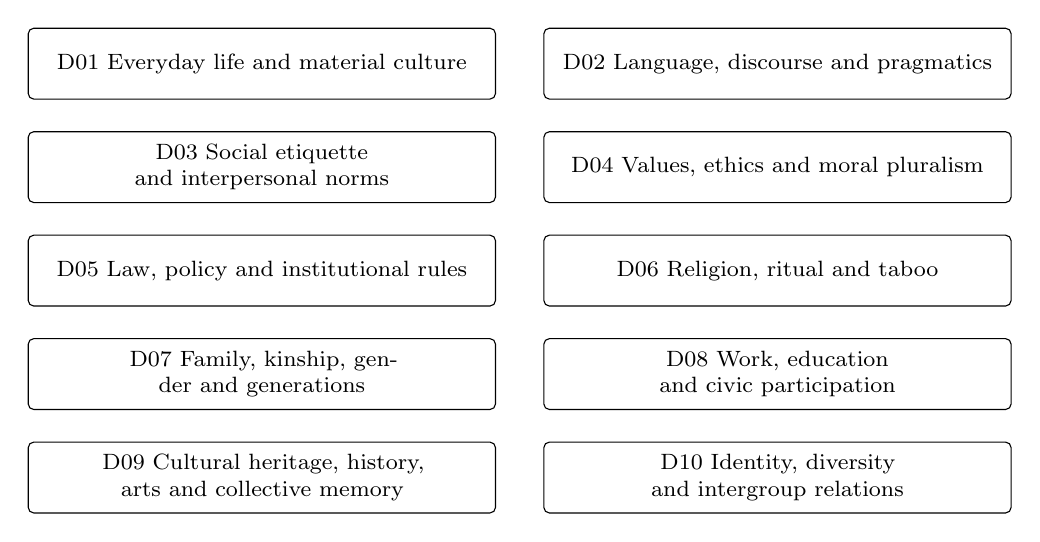
\begin{tikzpicture}[
  box/.style={draw, rounded corners=2pt, align=center, minimum height=9mm, text width=5.7cm, font=\footnotesize},
  node distance=4mm and 6mm
]
\node[box] (d1) {D01 Everyday life and material culture};
\node[box, right=of d1] (d2) {D02 Language, discourse and pragmatics};
\node[box, below=of d1] (d3) {D03 Social etiquette and interpersonal norms};
\node[box, right=of d3] (d4) {D04 Values, ethics and moral pluralism};
\node[box, below=of d3] (d5) {D05 Law, policy and institutional rules};
\node[box, right=of d5] (d6) {D06 Religion, ritual and taboo};
\node[box, below=of d5] (d7) {D07 Family, kinship, gender and generations};
\node[box, right=of d7] (d8) {D08 Work, education and civic participation};
\node[box, below=of d7] (d9) {D09 Cultural heritage, history, arts and collective memory};
\node[box, right=of d9] (d10) {D10 Identity, diversity and intergroup relations};
\end{tikzpicture}
\caption{The ten equally available diagnostic dimensions. The layout is presentational only and does not impose a hierarchy or fixed parent grouping.}
\label{fig:d01d10-framework}
\end{figure}


\section{The D01--D10 Dimensions}
\label{sec:dimensions}

\paragraph{D01 --- Everyday life and material culture.}
Everyday cultural competence often appears in mundane recommendations about meals, clothing, hospitality, celebrations, leisure or routines. BLEnD targets everyday cultural knowledge, while CANDLE includes food, clothing, traditions, rituals and behaviors among cultural-commonsense facets \parencite{myung2024blend,nguyen2023candle}. D01 captures such practical and material knowledge. It penalizes materially inappropriate guidance or unjustified universalization, but does not require stereotypical local markers to count as culturally adapted.

\paragraph{D02 --- Language, discourse and pragmatics.}
Cultural appropriateness is partly realized through how something is said. CARB includes cultural-linguistic evaluation, while intercultural pragmatics explicitly studies language use across cultural contexts and treats context, common ground, politeness and discourse as central to meaning \parencite{zhang2026carb,kecskes2014intercultural}. D02 therefore covers register, address forms, indirectness, implicature, idiom, humour and other interactional meanings. It is not a general writing-quality dimension; linguistic features matter here when they affect culturally situated interpretation or interpersonal fit.

\paragraph{D03 --- Social etiquette and interpersonal norms.}
D03 covers expectations governing greetings, invitations, gift giving, punctuality, disagreement, boundaries and related conduct. NormAd directly motivates this distinction by evaluating cultural adaptability across increasingly explicit social norms \parencite{rao2025normad}. The dimension asks whether advice recognizes relevant expectations without turning a tendency into a universal rule. It remains separate from D02 because socially inappropriate behavior can be expressed in linguistically natural language.

\paragraph{D04 --- Values, ethics and moral pluralism.}
Values concern judgments about desirable goals, rights and trade-offs rather than observable practice alone. CultureLLM uses World Values Survey material, while GlobalOpinionQA and cross-cultural bias research demonstrate variation in subjective opinions and value distributions \parencite{li2024culturellm,durmus2023globalopinionqa,tao2024culturalbias}. D04 covers contexts in which legitimate values can conflict. A high score therefore requires fair and context-sensitive treatment of relevant value pluralism, not the assumption that one majority preference represents unanimous morality.

\paragraph{D05 --- Law, policy and institutional rules.}
Formal rules require separate treatment because their authority differs from informal culture. SafeWorld explicitly combines geographically situated norms with laws and policies, and the reasoning framework of \textcite{wang2025ethicalreasoning} distinguishes formal constraints from social norms. D05 covers legal duties, institutional policies, rights and procedures. Its purpose is partly epistemic: a response should not present a formal requirement as merely ``what people usually do,'' or an informal convention as binding law.

\paragraph{D06 --- Religion, ritual and taboo.}
Religion and ritual combine factual, symbolic and normative content. UNESCO and CESCR include beliefs and traditions within broad accounts of cultural life, while CANDLE identifies ritual and tradition as recurring cultural facets \parencite{unesco2001culturaldiversity,cescr2009gc21,nguyen2023candle}. D06 covers observance, sacred meaning, ritual practice and context-dependent prohibitions. It explicitly avoids assuming uniform adherence within a religious community and rewards appropriate recognition of denominational, individual and situational variation.

\paragraph{D07 --- Family, kinship, gender and generations.}
Family relations are culturally variable and socially consequential. \textcite{georgas2006families} compare family networks, roles and emotional relations across thirty societies, while \textcite{inglehartnorris2003rising} document cross-national and generational variation in gender-role attitudes. D07 groups family structure, partnership, caregiving, gender relations, childhood, ageing and intergenerational expectations as an operational family/role domain. It penalizes categorical stereotypes or coercive assumptions and preserves individual agency and variation.

\paragraph{D08 --- Work, education and civic participation.}
Many culturally situated requests occur inside institutions. D08 covers workplaces, schools and universities, professional roles, associations and civic participation. \textcite{schwartz1999culturalvalues} develops a cultural-value framework with implications for work, while \textcite{inglehartbaker2000modernization} connect cultural change with values including tolerance, trust and participation. UNESCO and CESCR further connect education and participation with cultural life \parencite{unesco2001culturaldiversity,cescr2009gc21}. The dimension evaluates fit to the stated role, hierarchy, procedure and participation context without presuming one national institutional style.

\paragraph{D09 --- Cultural heritage, history, arts and collective memory.}
Historical and symbolic questions can carry identity and commemorative significance in addition to factual content. UNESCO and CESCR include heritage, traditions and artistic expression within cultural life \parencite{unesco2001culturaldiversity,cescr2009gc21}. \textcite{assmann1995collective} conceptualize cultural memory as socially transmitted collective knowledge and identity rather than biological inheritance. D09 therefore covers heritage, historical interpretation, commemoration, arts, public symbols and collective memory while retaining ordinary evidential standards for historical claims.

\paragraph{D10 --- Identity, diversity and intergroup relations.}
Cultural contexts intersect with national, regional, ethnic, linguistic, migration, disability, sexual and other identities. CultureBank's situated narratives and global-opinion research caution against reducing populations to homogeneous national profiles \parencite{shi2024culturebank,durmus2023globalopinionqa}. Pluralistic-alignment work similarly argues for preserving reasonable variation across populations \parencite{sorensen2024pluralistic}. D10 captures stereotyping, othering, discrimination and the representation of plural identities and intergroup relations.

\section{Scoring Anchors and Abstention}
\label{sec:framework-scoring}

Each applicable dimension receives one of three ordinal scores or an abstention. The scale is deliberately coarse: it distinguishes material misalignment, mixed or incomplete treatment, and appropriately contextualized treatment without manufacturing fine numerical precision. Dimension-specific runtime anchors specialize these general meanings.

\begin{table}[htbp]
\centering
\small
\caption{General interpretation of the D01--D10 scoring states.}
\label{tab:dimension-anchors}
\begin{tabular}{p{1.6cm}p{11.2cm}}
\toprule
\textbf{State} & \textbf{General interpretation} \\
\midrule
0 & Materially culturally misaligned: substantively wrong, inappropriate, stereotyping, misleading or incompatible with a material contextual constraint. \\
1 & Mixed, incomplete or context-limited: partly usable but oversimplified, insufficiently qualified or poorly adapted. \\
2 & Culturally aligned/appropriate: accurate, constructive and context-sensitive treatment of the applicable concern. \\
\texttt{abstain} & A defensible dimension judgment could not be established from the available basis; this is not a midpoint score. \\
\bottomrule
\end{tabular}
\end{table}

The scores are ordinal at dimension level. A 2 is a better rubric outcome than a 1, but it is not interpreted as ``twice as appropriate.'' Abstention is also distinct from 1: a mixed response has been evaluated and found partly appropriate, whereas abstention indicates insufficient basis for a valid score. Aggregation and coverage accounting are defined separately in \cref{ch:verifier}.

\section{Cultural Tendency, Rule, and Value}
\label{sec:tendency-rule-value}

A frequent cultural-evaluation error is using the wrong epistemic category. The framework therefore distinguishes four recurring forms. \emph{Descriptive tendencies} report common practices and require qualification about scope and variation. \emph{Interpersonal norms} describe socially expected conduct but may vary by relationship, generation, region or subgroup; NormAd demonstrates why this contextual specificity matters \parencite{rao2025normad}. \emph{Formal rules} derive from law, policy or institutional authority and can impose obligations regardless of social preference. \emph{Values and contested judgments} concern what people regard as desirable, fair or respectful; cross-national opinion work shows that these distributions can vary substantially \parencite{durmus2023globalopinionqa,tao2024culturalbias}.

These categories can co-occur. A question about religious accommodation at work may involve D06 religious practice, D08 institutional context and D05 formal rules. The framework permits multiple applicable dimensions because its purpose is diagnostic coverage rather than mutually exclusive cultural classification.

\section{Framework Limitations}
\label{sec:framework-limitations}

The D01--D10 framework remains a designed operationalization. The literature supports the relevance of its component facets but does not establish that ten dimensions are uniquely correct or exhaustive. The dimensions also overlap: language can express identity, religion can shape family expectations, workplace advice can involve law, and historical memory can affect intergroup relations. Dimension-level results should therefore not be interpreted as statistically independent constructs without further validation.

A second limitation follows from prompt-level planning. Using one shared plan improves comparability across four candidates, but a candidate can introduce a culturally problematic topic that the prompt itself did not make salient. The present method records this as a limitation rather than dynamically changing the plan per candidate.

Finally, the rubric does not guarantee evaluability. Cultural evidence is unevenly available across regions, languages and communities, and some knowledge is tacit or contested. A culturally appropriate answer is also not synonymous with conformity to a majority tendency. The framework preserves pluralism, rights, agency and contextual variation by design. Whether this operationalization aligns with human judgments is therefore not assumed here; it is evaluated empirically in \cref{ch:experiment} and, once available, \cref{ch:results}.

\chapter{The Proposed Evidence-Grounded Cultural Verifier}
\label{ch:verifier}

The previous chapter operationalized cultural appropriateness as a multidimensional and context-sensitive construct. This chapter defines the method used to evaluate one generated response against that construct. The central design goal is not to turn external retrieval into a second language-model opinion, but to separate three functions that are often conflated in automated evaluation: identifying what in a response is materially relevant, acquiring evidence about externally checkable cultural claims, and assigning a final rubric-based judgment. The resulting verifier is a standalone post-hoc evaluation system. It does not use reward-model scores, human reference labels, benchmark answers or expected-error annotations as inputs.

The implementation on the frozen \texttt{agent/final-verifier} branch follows the sequence
\[
\begin{aligned}
\text{prompt} &\rightarrow \text{context} \rightarrow \text{dimension plan} \rightarrow \text{material targets} \\
&\rightarrow \text{verification questions} \rightarrow \text{evidence} \rightarrow \text{frozen memo} \\
&\rightarrow \text{target verdicts} \rightarrow \text{dimension scores} \rightarrow \text{aggregate score}.
\end{aligned}
\]
For Best-of-4 evaluation, the prompt-level context and dimension plan are shared across all four candidates, while all candidate-dependent stages are executed independently. The verifier therefore produces both a scalar ranking signal and a diagnostic trace explaining which dimensions, targets and evidence contributed to the result.

\section{Design Objectives}
\label{sec:verifier-objectives}

The verifier is guided by seven methodological objectives. First, it must remain \emph{independent of the systems against which it is compared}. Reward-model outputs, direct-judge preferences and human labels are therefore excluded from the verifier interface. Second, cultural interpretation must be \emph{context-sensitive}. Prior work on social norms and geo-diverse safety shows that the same behavior can be interpreted differently depending on explicit setting, relationship, location or institutional constraints \parencite{rao2025normad,yin2024safeworld,wang2025ethicalreasoning}. The pipeline therefore extracts supported prompt context before selecting applicable rubric dimensions.

Third, externally checkable claims should be distinguished from purely internal qualities or non-verifiable value statements. This prevents unnecessary search for issues that must be judged from the response itself. Fourth, evidence acquisition should be separated from the final candidate comparison as far as the task permits. LLM-based evaluators are known to exhibit order and framing effects in comparative settings \parencite{zheng2023llmjudge,wang2024notfairevaluators}; this motivates a structural boundary after verification-question generation, although it does not establish that the resulting evidence stage is unbiased. Fifth, the search process must be bounded and auditable. Retrieval introduces freshness and provenance advantages, but also contamination and search-opportunity risks \parencite{lewis2020rag,deng2024contamination}. The method therefore caps target and retrieval budgets, records every query and preserves the exact evidence used.

Sixth, the verifier must be able to express \emph{insufficient basis}. A forced cultural score can be misleading when evidence is missing or structurally invalid. The system therefore supports dimension-level abstention and reports coverage separately from score, conceptually related to the broader reject-option principle in selective prediction \parencite{geifman2017selective}. It does not, however, inherit formal risk guarantees from selective-classification algorithms. Seventh, every completed judgment should be reconstructable from an execution trace containing model configuration, prompt-template versions, retrieved documents, identifiers and stage outputs.

These objectives are implemented as explicit data and control-flow constraints rather than as informal prompting alone. Table~\ref{tab:verifier-stages} summarizes the main stages and their principal inputs.

\begin{table}[htbp]
\centering
\footnotesize
\setlength{\tabcolsep}{3pt}
\renewcommand{\arraystretch}{1.08}
\caption{Main stages of the standalone cultural verifier.}
\label{tab:verifier-stages}
\begin{tabular}{p{3.2cm}p{4.4cm}p{5.7cm}}
\toprule
\textbf{Stage} & \textbf{Primary input} & \textbf{Output / methodological role} \\
\midrule
Context extraction & Prompt & Explicitly supported contextual facts with verbatim prompt spans \\
Dimension planning & Prompt, context, D01--D10 rubric & Shared applicable-dimension plan with one primary dimension when nonempty \\
Target extraction & Prompt, response, context, plan & Up to three decision-relevant response targets with epistemic type and exact quote \\
Question generation & Target, context & Baseline and variation questions that remove candidate identifiers and evaluative framing \\
Blind evidence stage & Questions, context & Queries, retrieved documents, source classes and evidence memo \\
Target comparison & Target, frozen memo & Supported, contradicted, mixed or insufficient verdict \\
Dimension scoring & Full response, plan, targets, verdicts, memos, rubric & D01--D10 scores in \{0,1,2,abstain\} \\
Aggregation/ranking & Non-abstained scores & Equal-weight overall score and exact Best-of-4 comparison \\
Trace & All stage artifacts & Reconstructable record of configuration, calls, links, errors and result \\
\bottomrule
\end{tabular}
\end{table}

\section{Overall Architecture and Semantic Backbone}
\label{sec:overall-architecture}

All semantic stages use one explicitly configured language model. The implementation rejects a mismatch between the model configuration attached to the adapter and the configuration attached to the pipeline. The same provider, model identifier and temperature are therefore used for context extraction, dimension planning, target extraction, question generation, query rewriting, source classification, memo synthesis, follow-up generation, target comparison and dimension scoring. This design reduces one source of uncontrolled heterogeneity: differences between stages cannot silently be attributed to different model backbones.

The configuration does not provide a scientifically preferred default model. A model identifier must be supplied explicitly, and the current local \texttt{qwen3:4b} setting is a development convenience rather than the final experimental choice. The supported built-in providers are Ollama and OpenRouter, with a custom-adapter interface for alternatives. OpenRouter requests disable provider fallback, so a nominal model cannot silently be replaced by another backend model. Temperature defaults to zero, but this is treated only as a variance-reduction setting; it does not imply perfect determinism.

Semantic calls are stateless. Every request contains a fresh system message and a serialized payload rather than accumulated chat history. The semantic session records each attempt, validates the model output against a strict Pydantic schema and applies at most one semantic repair retry. Transport-level retries are separately bounded. A failure after those budgets raises a structured stage error rather than allowing an unvalidated value to continue through the pipeline. This distinction between semantic generation and Python validation is central to the method: Python enforces format, identifiers, exact quotations, evidence links and budgets, but it does not hard-code which cultural conclusion or score is correct.

\section{Context Extraction}
\label{sec:context-extraction}

The first semantic stage sees only the user prompt. It extracts a \texttt{ContextFrame} containing the setting, participants, relationships, explicit location, temporal context, explicit constraints and user goal. Each non-null contextual fact contains both a normalized value and an exact \texttt{prompt\_span}. The validator requires that this span occur verbatim in the original prompt. As a result, a model-generated statement such as an inferred nationality or religion cannot pass validation unless the prompt itself contains an exact supporting span.

The prompt instruction further prohibits demographic inference from names and prohibits assuming a default country. These instructions are not in themselves a guarantee against hallucination; the stronger implementation property is that every retained fact must be traceable to verbatim prompt text. If context extraction remains structurally invalid after its bounded retry, the planner replaces it with an empty context frame. This fallback is intentionally conservative: unsupported context is discarded instead of being repaired by inserting a plausible but ungrounded assumption.

An empty context does not automatically terminate evaluation. Dimension planning can still proceed from the prompt. Conversely, if the planning stage itself fails, the candidate evaluation is treated as a pipeline failure rather than as a culturally neutral response. This separation is useful because uncertainty about context and failure to execute the evaluation are methodologically different events.

\section{Prompt-Level Dimension Planning}
\label{sec:dimension-planning}

The planner receives the prompt, the validated context frame and the full D01--D10 rubric from \cref{ch:framework}. It selects the dimensions that are applicable to the prompt and assigns exactly one of them the role \texttt{primary} when the plan is nonempty; any others are marked \texttt{secondary}. The roles describe relevance, not score weight. Aggregation later treats all scored dimensions equally.

The plan is produced before any candidate response is inspected. This is especially important in Best-of-4 mode. The \texttt{rank} interface computes one context frame and one dimension plan from the prompt and passes those identical objects to all four candidate evaluations. Candidate A therefore cannot be scored on a different prompt-level rubric simply because it mentions a different culturally salient detail than candidate B. This improves comparability across the set and prevents the evaluator from selecting more favorable dimensions for one candidate after seeing its answer.

The design also has a known limitation. A response can introduce a cultural issue that was not salient in the prompt-level plan. Because target dimensions must be a subset of the planned dimensions, that issue may not become an independently scored dimension. The final dimension scorer does see the complete response and can consider omitted explicit requirements, but the frozen method does not dynamically expand the prompt-level dimension set per candidate. This trade-off between cross-candidate comparability and candidate-specific coverage is reported explicitly rather than hidden by adaptive planning.

\section{Material Target Extraction}
\label{sec:target-extraction}

Once a shared plan exists, the verifier analyzes one candidate response and extracts a bounded set of \emph{material targets}. A target is a decision-relevant unit whose correctness or contextual suitability could materially affect the cultural judgment. The semantic instruction asks for normally one or two such units and permits at most three. The cap prevents long answers from gaining effectively unlimited search opportunities and keeps evidence acquisition comparable across candidates.

Each target stores five substantive elements: an exact quotation from the candidate response, a normalized proposition, an epistemic type, the relevant planned dimension identifiers and a materiality explanation. Exact response quotations are validated against the original response. Target references to dimensions outside the prompt-level plan are rejected. If the extractor identifies more material units than the budget can represent, it can set \texttt{targets\_truncated=true}; this exposes the coverage limitation instead of silently pretending that the response has been exhaustively decomposed.

The epistemic type determines whether external retrieval is appropriate. The runtime schema distinguishes five classes: external facts; descriptive cultural norms; context-dependent recommendations; response-internal quality; and non-verifiable value statements. Their serialized labels are shown below:
\begin{center}
\small
\texttt{external\_fact}, \texttt{descriptive\_cultural\_norm}, \texttt{context\_dependent\_recommendation}\\
\texttt{response\_internal\_quality}, \texttt{non\_verifiable\_value\_statement}.
\end{center}
Internal-quality and non-verifiable-value targets are structurally forbidden from triggering retrieval. Externally checkable facts, descriptive norms and context-dependent recommendations may be routed to the evidence pipeline. This avoids the category error of searching the web to decide, for example, whether a response is internally coherent or whether a purely normative preference is objectively true.

Target extraction is quote-based, which creates a second limitation. A missing requirement in the response has no response span from which to form a target. The dimension scorer therefore receives the full prompt and response and is instructed to consider omitted explicit requirements at scoring time, but omissions do not receive their own target-level retrieval trace in the current method.

\section{Neutral Verification Questions}
\label{sec:verification-questions}

For each retrievable material target, the verifier generates exactly two initial questions in a fixed order: a \texttt{baseline} question and a \texttt{variation} question. The baseline question asks what is documented about the underlying subject; the variation question asks what contextual variation or scope qualifications matter. The intent is to discourage a single retrieved source from being converted into an unjustified universal rule, which is particularly important for cultural practices and social norms. Prior work on community-grounded cultural knowledge and cross-national opinions motivates explicit attention to variation rather than one monolithic profile \parencite{shi2024culturebank,durmus2023globalopinionqa}.

Question generation necessarily sees the material target. This fact places a precise boundary on what can be called \emph{candidate-blind}. The generator must know the proposition under investigation in order to ask useful evidence questions. Its instruction therefore attempts to remove candidate wording, identifiers and evaluative language and to avoid requesting proof that the candidate is correct or incorrect. However, the generated question can still preserve framing inherited from the target. The thesis consequently does not describe the full pipeline as end-to-end blind and does not claim that neutral-question prompting eliminates framing bias.

The stronger structural claim begins only after these two questions have been created. The target identifier, response text, candidate position and target verdict are not included in the question objects passed to the evidence engine.

\section{Candidate-Blind Evidence Boundary}
\label{sec:blind-boundary}

The evidence engine exposes a deliberately narrow public interface: it accepts exactly a tuple of two \texttt{VerificationQuestion} objects and one \texttt{ContextFrame}. Runtime checks reject subclassed or lookalike containers that might carry extra candidate fields. The underlying Pydantic models also forbid unknown fields. Candidate text, material-target objects, candidate letters, human labels, reward-model outputs and target verdicts are therefore unavailable to the query-rewriting, retrieval, source-classification and evidence-synthesis stages through this interface.

The engine also creates a fresh semantic session. No preceding candidate conversation state is retained. This is an implementation mechanism for reducing direct candidate-conditioned evidence interpretation: after the questions are formed, the evidence subsystem cannot simply reread the answer and search for sources that support its wording. The design responds to known concerns about LLM-evaluator sensitivity to comparison context and presentation order \parencite{zheng2023llmjudge,wang2024notfairevaluators}, but the literature does not validate this exact architectural mechanism and the implementation does not prove the absence of bias.

Two residual channels remain. First, the verification questions originate from candidate-derived targets and can therefore carry framing. Second, retrieved web content can itself be selective, biased or incomplete. Candidate blindness should thus be interpreted as a controlled information boundary, not as a guarantee of epistemic neutrality.

\section{Query Rewriting and Evidence Retrieval}
\label{sec:retrieval}

Each verification question is rewritten into one search query using only the question and the validated context. The query-rewriter does not receive the response or target object and is instructed not to add a verdict. Search is performed in LIVE mode through a Tavily adapter. The current adapter requests general search with \texttt{search\_depth=advanced} by default and explicitly disables generated answers, raw-page content and images.

The resulting evidence unit is therefore a search-result excerpt rather than a fully downloaded web page. For every accepted document, the system records a stable document identifier, the originating query, URL, title, excerpt text, rank, provider score when available, retrieval timestamp, content hash and later a semantic source class. This distinction is important: the thesis can claim that the verifier preserves the search content it actually used, but it cannot claim to have parsed or verified the full underlying webpage.

The retriever requests up to twice the configured \texttt{top\_k} results, subject to an implementation maximum of twenty, so that provenance filtering and deduplication can remove unsuitable entries before the final budget is applied. At most \texttt{top\_k} accepted documents are retained per question; the frozen default is three. Fewer may remain after filtering. Retrieval is therefore bounded both by the target budget and by the per-question document budget.

The use of retrieval follows the general motivation of retrieval-augmented systems: explicit external evidence can provide provenance and can be refreshed independently of model parameters \parencite{lewis2020rag}. In this thesis, however, retrieval is not used to improve the generated answer. It is an evaluation-stage evidence source, and empirical accuracy still depends on whether the queries retrieve relevant and representative material.

\section{Leakage and Contamination Filtering}
\label{sec:leakage-filtering}

Because the evaluation repository itself contains prompts, annotations and research artifacts, search results must not be allowed to reveal known benchmark answers or provisional labels. Before any evidence reaches the semantic synthesis stage, the retrieval layer applies provenance exclusions. The default configuration excludes the thesis repository on GitHub and common annotation or result paths, while additional domains, repositories and URL/path globs can be frozen for the final experiment.

Filtering occurs before source classification and memo generation. Canonicalized URLs and content hashes are also used for deduplication. Every rejected result is stored with a reason such as excluded domain, excluded repository, excluded path or duplicate URL/content. Accepted snapshots are integrity-checked against their content hashes, and a frozen snapshot that later violates the active exclusion policy causes an explicit error.

These controls are motivated by the broader problem of benchmark contamination, which can inflate apparent evaluation performance \parencite{deng2024contamination}. Their scope is deliberately limited. URL and repository rules can block known answer-bearing sources; they cannot prove that an unknown mirror does not contain the same material, nor can they remove information learned during the verifier model's pretraining. The exclusion list must therefore be reviewed and frozen before held-out evaluation, and leakage filtering is reported as a mitigation rather than a contamination guarantee.

\section{Source Classification}
\label{sec:source-classification}

Accepted documents are classified semantically into eight source families: official/legal, academic peer-reviewed, statistical survey, institutional/professional, community insider, general explanatory, commercial/lifestyle, or unknown. The implementation serializes these as:
\begin{center}
\small
\texttt{official\_legal}, \texttt{academic\_peer\_reviewed}, \texttt{statistical\_survey}, \texttt{institutional\_professional}\\
\texttt{community\_insider}, \texttt{general\_explanatory}, \texttt{commercial\_lifestyle}, \texttt{unknown}.
\end{center}
Every document must receive exactly one classification, and the classifier is instructed not to infer peer review merely from formal writing style.

The classes are not converted into a universal numerical quality score. Source fitness depends on the question. An official primary source is normally preferable for a binding legal rule; empirical linguistic research may be better suited to a pragmatic convention; and credible community evidence can be informative for lived practice that is poorly represented in formal institutions. The evidence-memo prompt is instructed to reason about this fit rather than to treat one source class as globally superior.

Classification itself remains an LLM judgment. Python validates that each document is classified exactly once and that document identifiers match, but it does not verify that a source truly is peer reviewed or institutionally authoritative. Misclassification is therefore a semantic failure mode to be audited empirically.

\section{Candidate-Blind Evidence Memo}
\label{sec:evidence-memo}

After the initial questions have been searched and the documents classified, the evidence model synthesizes an \texttt{EvidenceMemo}. The memo contains an answer, scope statement, variation statement, agreement/disagreement description, a sufficiency state, a confidence category, structured evidence statements and citations. Sufficiency is one of \texttt{sufficient}, \texttt{conflicting} or \texttt{insufficient}; confidence is \texttt{low}, \texttt{medium} or \texttt{high}.

Each factual evidence statement is explicitly categorized as a tendency, context-sensitive practice, legal/institutional rule, or universal claim. The corresponding serialized labels are \texttt{tendency}, \texttt{context\_sensitive\_practice}, \texttt{legal\_institutional\_rule}, and \texttt{universal\_claim}. This mirrors the epistemic distinctions introduced in \cref{sec:tendency-rule-value}: a common practice should not silently become an obligation, and one local convention should not become a universal cultural truth. The memo instruction also requires unresolved disagreements to remain visible rather than being collapsed into artificial consensus.

Citation structure is programmatically checked. Every citation must refer to an actually retrieved document identifier, the union of statement-level citations must equal the memo's overall citation set, and a memo marked sufficient or conflicting must contain citations. If no documents are available, the only structurally valid state is insufficient evidence with low confidence. These constraints make fabricated identifiers or uncited factual claims harder to pass through the pipeline.

They do not prove semantic entailment. A cited source can be misread, an excerpt can omit decisive context, and the LLM can draw an unsupported inference even when the document identifier is valid. The distinction between citation integrity and evidence correctness is therefore maintained throughout the thesis. Human-grounded evaluation and trace inspection are required to determine whether the memo is substantively reliable.

\section{Bounded Follow-Up}
\label{sec:bounded-followup}

The first evidence round always consists of the two initial questions. After the first memo is synthesized, one additional retrieval opportunity is available only when the memo is not marked \texttt{sufficient} and the configured maximum number of rounds is two. A follow-up stage may then generate one neutral, gap-specific question, or it may return no question if further search is unlikely to help. If a follow-up is generated, it is searched once, the new documents are added and a final memo is synthesized from all evidence. Search then terminates.

This bounded policy serves three purposes. It limits cost, it prevents one difficult candidate from receiving an arbitrarily larger evidence-search budget, and it makes the search process easier to reproduce. The value of one optional follow-up is a design decision, not an empirically established optimum. The final experiment can assess its practical consequences, but the methodology does not claim that two retrieval rounds maximize cultural accuracy.

\section{Evidence Freezing}
\label{sec:evidence-freezing}

A central ordering constraint is that evidence is finalized before the candidate proposition is reintroduced. The final \texttt{EvidenceMemo} is an immutable Pydantic object. The pipeline records a \texttt{memo\_frozen} event, computes a cryptographic digest of the memo, and only then passes the target and memo to the target-comparison stage. After comparison, the digest is computed again; any change raises an error. Trace validation also checks the links among target, questions and final memo.

Freezing prevents a later comparator from rewriting the evidence summary after learning what the candidate actually claimed. It is therefore an implementation-level anti-post-hoc-editing mechanism. The thesis does not infer from this ordering alone that accuracy increases or bias disappears. The empirical contribution of this separation is one of the properties to be examined in the final comparative evaluation and qualitative error analysis.

\section{Target Comparison}
\label{sec:target-comparison}

Only after the memo has been frozen does the comparator receive the material target again. It evaluates the proposition against that memo and returns one of four verdicts: \texttt{supported}, \texttt{contradicted}, \texttt{mixed} or \texttt{insufficient}. The verdict must contain the exact target identifier and memo identifier, which are validated before the result can be used downstream.

The comparator instruction explicitly states that missing evidence is not contradiction and that scope and contextual variation matter. This is important in cultural evaluation because absence of evidence for a practice is not evidence that the practice is culturally wrong, and evidence of a common tendency does not imply a universal rule.

A target verdict is not itself a cultural score. A response can contain a factually contradicted statement whose cultural relevance is minor, or a factually supported statement that is nevertheless inappropriate in the user's context. The dimension scorer therefore receives the verdict as one diagnostic input rather than applying a hard-coded mapping such as ``contradicted implies zero.''

\section{D01--D10 Dimension Scoring}
\label{sec:dimension-scoring}

The final semantic judgment is performed at dimension level. The scorer receives the original prompt, the full candidate response, validated context, frozen dimension plan, material targets, target verdicts, final evidence memos and the complete D01--D10 rubric. It must return exactly one score for every planned dimension and no score for an unplanned dimension.

The possible outcomes are 0, 1, 2 or \texttt{abstain}, using the anchors defined in \cref{sec:framework-scoring}. The scorer is instructed to distinguish supported factuality from cultural appropriateness: a supported claim does not automatically deserve a high cultural score, and a contradicted target does not automatically force a zero. It must explain the material cultural relevance of the available evidence and preserve distinctions among common practice, obligation and preference.

Every non-abstained score for a nonempty response must contain at least one exact response quotation. Any referenced target or memo identifier must exist, and the validator checks that the referenced target is linked to the dimension being scored. Memo references are likewise accepted only when the memo belongs to a target associated with that dimension. These checks make it possible to reconstruct why a dimension received a score and reduce the risk of free-floating rationales that cite unrelated evidence.

Python does not validate whether a score of 0, 1 or 2 is semantically correct. If the scorer repeatedly returns structurally invalid output, or if an upstream stage fails, the candidate result receives \texttt{status=failed} and the applicable dimensions are represented as abstentions with an explicit failure rationale rather than fabricated scores. This failure state must be distinguished empirically from a legitimate completed evaluation that abstains because the evidence basis is insufficient.

\section{Aggregation and Coverage}
\label{sec:aggregation}

Dimension scores are aggregated without primary/secondary weighting. Let $J$ be the set of applicable dimensions that received a numeric score, with $s_d \in \{0,1,2\}$ for dimension $d$. The candidate score is
\begin{equation}
S = \frac{1}{|J|}\sum_{d \in J}\frac{s_d}{2},
\label{eq:verifier-score}
\end{equation}
which lies in $[0,1]$. If $J$ is empty, the overall score is \texttt{null} and the candidate is marked abstained. Internally, the implementation uses exact rational arithmetic for comparison and converts the result to a floating-point value only for the stored candidate output.

Abstained dimensions are excluded from the mean. This makes the score interpretable as performance on dimensions the system actually judged, but it introduces a comparability issue: two candidates can have equal means over different subsets of dimensions. The result therefore records \texttt{applicable\_count}, \texttt{scored\_count} and the identifiers of abstained dimensions.

The pipeline also reports \texttt{evidence\_coverage}. If $T_R$ is the number of material targets marked retrieval-appropriate and $T_S$ the number whose final evidence memo is marked \texttt{sufficient}, then
\begin{equation}
C_E = \frac{T_S}{T_R}
\end{equation}
when $T_R>0$; otherwise evidence coverage is \texttt{null}. This metric describes sufficiency coverage, not factual accuracy. A sufficient memo can still be semantically wrong, and a candidate requiring no external evidence is not assigned artificial perfect coverage.

\section{Best-of-4 Ranking}
\label{sec:bestof4-ranking}

The public ranking interface requires exactly four responses. As described in \cref{sec:dimension-planning}, context extraction and dimension planning occur once from the shared prompt. Each candidate is then evaluated independently under that same plan, with a fresh semantic session and its own targets, evidence bundles, verdicts, scores and trace.

Ranking uses the exact rational aggregate rather than rounded floating-point output. Among candidates with non-null scores, the highest exact value wins only if it is unique. If two or more candidates share the exact maximum, the system returns \texttt{no\_clear\_winner}; if all four candidates abstain, it likewise returns \texttt{no\_clear\_winner}. No arbitrary epsilon or tie margin is introduced.

The ranking result also exposes \texttt{coverage\_comparable}, which is true when all candidates were scored on the same set of dimensions. The frozen ranking rule does not override the highest-score winner when coverage differs. Consequently, a candidate scored on fewer dimensions can in principle obtain a higher mean than a candidate with broader coverage. This is a known limitation and motivates reporting score together with coverage and abstention rather than interpreting the winner label in isolation.

Execution failure is also kept separate from a substantive tie. A failed candidate generally produces no numeric overall score; if other candidates have valid scores, ranking proceeds among the available non-null scores. The final experiment therefore reports system failures separately from cultural abstentions and ranking outcomes.

\section{LIVE and REPLAY Modes}
\label{sec:live-replay}

Evidence acquisition is divided into LIVE and REPLAY modes to separate collection of web evidence from repeated semantic evaluation. In LIVE mode the Tavily retriever is active. Each query produces an immutable retrieval snapshot stored under the evidence-cache directory. The snapshot contains the accepted documents, filtered results, provider identity, query object and a hash of the retrieval configuration. The system also stores an evidence schedule containing the initial questions, any follow-up question, exact queries, snapshot identifiers and snapshot hashes.

An existing schedule is reused when its key matches the current questions, context, retrieval configuration, provider/model configuration, temperature and prompt-template digest. A genuinely new evidence collection should therefore use a new cache directory rather than silently overwriting frozen artifacts. This preservation step is part of the experimental protocol in \cref{ch:experiment}.

In REPLAY mode the verifier does not retain a live retriever at all. It loads the frozen schedule and snapshots, verifies their identifiers, hashes, questions, queries and active leakage policy, and fails explicitly if material is missing or inconsistent. There is no live-search fallback. Query rewriting is not repeated for a frozen schedule; the stored queries are reused.

REPLAY freezes the evidence acquisition path, not the whole semantic pipeline. Prompt-level context, planning and initial question generation are still semantic operations, and evidence memos, target comparison and dimension scoring still invoke the configured model. If nondeterminism changes the context or questions such that the frozen schedule no longer matches, replay fails rather than substituting a different search. Temperature zero and fixed evidence therefore reduce variability but do not guarantee bit-for-bit identical final judgments.

\section{Traceability and Reproducibility}
\label{sec:traceability}

Every candidate evaluation writes a JSON trace to the configured trace directory. The trace records a run identifier, pipeline version, Git commit when available, UTC timestamp, LIVE/REPLAY mode, serialized configuration, hashes of the prompt, response, rubric and prompt templates, template versions, semantic call records, target-to-evidence links, ordering events, the complete candidate result and partial evidence state when a failure interrupts execution.

Each semantic call record contains the stage name, attempt number, timestamp, input hash, structured output JSON when available and an error category when the attempt fails. API keys are not members of the configuration schema and are therefore not serialized into the trace. The top-level trace stores hashes rather than plain prompt and response fields; nevertheless, exact prompt spans, response quotations and semantic outputs contained deeper in the result can reproduce fragments of the original text. Traces should therefore be treated as research data rather than as automatically anonymized artifacts.

Stable identifiers are derived from canonical JSON hashes for targets, questions, queries, documents, memos and snapshots. Atomic JSON writes reduce the risk of partially written artifact files. Trace validation then checks cross-object consistency: every verdict must link to an existing target and memo, every memo citation must refer to an available document, every query must match its snapshot, every content hash must match its text and every completed retrievable target must have a verdict. These properties support auditability and rerunning, but they do not substitute for semantic inspection of whether the evidence and cultural reasoning are substantively correct.

\section{Implementation Verification}
\label{sec:implementation-verification}

The frozen implementation was validated as software before the final empirical study. In the recorded Python 3.12 environment, the active suite reports 55 passing tests and one explicitly gated live-provider test skipped. Ruff linting and format checks also pass. The tests cover context-span validation and recovery, D01--D10 rubric loading, target budgets, question shape, candidate-blind call boundaries, query inputs, source citations, provenance filtering, duplicate evidence, memo immutability, bounded follow-up, aggregation, abstention, exact ties, shared Best-of-4 planning, REPLAY integrity, failure traces, provider contracts, CLI behavior and package installation.

These checks establish that the software follows its intended contracts under deterministic fixtures and mocked network boundaries. They do not establish cultural validity, evidence accuracy or superiority to reward models or direct LLM judging. The only end-to-end real-provider LIVE-to-REPLAY smoke test is intentionally gated and was not executed in the validation snapshot because final model/provider credentials were not configured. More importantly, no unit-test suite can answer the thesis's empirical research questions. Those require the held-out human-grounded comparison defined in \cref{ch:experiment}.

\section{Methodological Summary and Residual Limitations}
\label{sec:verifier-summary}

The verifier's methodological contribution is the composition of several explicit boundaries: prompt-supported context before interpretation, shared prompt-level dimension planning, bounded target decomposition, candidate-derived but neutralized verification questions, a structurally candidate-blind evidence stage, provenance-filtered retrieval, source-aware evidence synthesis, one bounded follow-up, evidence freezing before target comparison, dimension-level abstention and exact equal-weight aggregation. The system is therefore more than a scalar judge, because it produces inspectable intermediate objects and preserves the evidence path that led to each decision.

The same architecture leaves identifiable limitations. Candidate information can influence question wording before the blind boundary. Search uses provider excerpts rather than full documents. Source classification and evidence synthesis remain model judgments. Quote-based targets do not independently represent omissions. The shared prompt-level plan can miss candidate-introduced dimensions. Evidence coverage and scoring coverage can differ across candidates. REPLAY fixes retrieval artifacts but not language-model nondeterminism. Finally, no implementation constraint guarantees that the selected evidence represents a culture fairly or that a dimension score agrees with human judgment.

These limitations are not exceptions to the method but part of its empirical evaluation target. The next chapter therefore freezes the experimental protocol needed to compare the standalone verifier with human reference judgments, the independent Skywork reward-model baseline and a direct LLM-as-a-judge baseline without allowing any of those comparators to influence the verifier itself.

\chapter{Experimental Design and Evaluation Protocol}
\label{ch:experiment}

This chapter defines the protocol for evaluating the standalone verifier against an external human reference and two independent baselines. The study is designed to answer whether the verifier agrees with human judgments, how that agreement compares with a preference-based reward model and a direct LLM judge, and what additional diagnostic information is provided by evidence grounding, abstention, and dimension-level scoring. Methodological choices are fixed before final comparative results are inspected. Values that are not yet scientifically frozen---most importantly the final semantic model, direct-judge configuration, and completed human annotations---remain explicit placeholders rather than being inferred from development runs.

\section{Evaluation Objectives}

The experiment maps directly to the research questions. RQ1 measures agreement between verifier and human reference judgments. RQ2 compares the verifier with Skywork-Reward-V2 and a direct LLM-as-a-judge baseline on the same Best-of-4 items. RQ3 analyzes verifier-specific diagnostics such as D01--D10 scores, evidence coverage, abstention, material targets, and evidence traces. RQ4 examines trace-backed failure modes in retrieval, question framing, target extraction, planning, and scoring.

The primary empirical target is therefore agreement with the aggregated human reference, not agreement with CARB, provisional AI labels, or raw reward scores. The human reference is itself treated as an aggregated judgment rather than as objective cultural truth, consistent with pluralistic views of value alignment and cultural modeling \parencite{sorensen2024pluralistic,adilazuarda2024culture}.

\section{Evaluation Dataset}
\label{sec:eval-dataset}

The project contains 30 Best-of-4 candidate sets, \texttt{PLT001}--\texttt{PLT030}. Each set contains one prompt and four preserved candidate responses. The long-format source records candidate positions C1--C4, generator provenance, and the generator model \texttt{llama3.2:3b}; a project script converts the data to one row per prompt with responses A--D. The same project also contains older provisional annotations labeled \texttt{synthetic\_model\_provisional} and \texttt{requires\_human\_verification}. These labels are development artifacts only and are excluded from the human reference and from all evaluated systems.

Because the PLT items existed during the broader development process, the thesis will not automatically describe them as a strictly unseen held-out test set. Unless a provenance audit establishes otherwise, the scientifically accurate term is \emph{fixed evaluation set}. If an additional unseen confirmatory set is created before the final experiment, it will be reported separately. No item may be excluded after inspecting system outcomes; exclusions are allowed only for pre-declared structural problems such as a missing response or corrupted prompt and must be documented.

\section{Best-of-4 Candidate Setup}

For item $i$, the systems receive one prompt $p_i$ and four fixed responses $(r_{iA},r_{iB},r_{iC},r_{iD})$. Candidate text is never regenerated between baselines. The verifier uses one shared prompt-derived context and dimension plan for A--D and then evaluates candidates independently. Skywork scores each prompt--response pair separately. The direct judge receives the prompt and all four candidates in one comparison request.

Candidate order is logged explicitly. The historical annotation materials preserve A--D order; therefore the thesis will report fixed human-survey order unless the final survey export proves that randomization was used. For the direct judge, a deterministic pre-generated permutation schedule will be frozen before execution and mapped back to canonical A--D labels, reducing systematic position effects while remaining reproducible. Order control is motivated by documented position bias in LLM evaluation \parencite{wang2024notfairevaluators}.

\section{Human Evaluation}
\label{sec:human-eval}

Five student annotators are planned. For each item, annotators see the prompt and complete responses A--D and answer: \emph{Which response is the most culturally appropriate?} The choices are A, B, C, D, and \emph{No clear winner}. A second required question records confidence from 1 to 5. The interface must not expose verifier outputs, reward-model scores, provisional labels, expected issues, benchmark answers, or evidence traces.

The annotators are not described as cultural experts unless their actual qualifications justify that description. The resulting label is therefore called a \emph{human reference judgment}, not cultural ground truth.

\subsection{Reference aggregation and agreement}

Primary aggregation uses unweighted categorical votes. Confidence does not weight the vote because no calibration model justifies treating higher self-reported confidence as greater correctness. With five annotators, at least three identical votes define a majority. A majority for A--D yields that candidate as reference winner; a majority for \emph{No clear winner} yields the corresponding reference category. If no option reaches three votes, the item is labeled \emph{unresolved human split} and excluded from primary winner-agreement accuracy while remaining in the disagreement analysis.

Raw agreement is reported together with a chance-corrected reliability statistic. If every item has a complete five-rater nominal matrix, Fleiss' $\kappa$ is used \parencite{fleiss1971kappa}. If ratings are missing or the matrix is unbalanced, nominal Krippendorff's $\alpha$ is used instead \parencite{krippendorff2018content}. This decision rule is based on the realized annotation structure, not on which statistic produces the more favorable value. Per-item vote distributions and confidence summaries are retained for later error analysis.

\section{Standalone Verifier Configuration}

The experimental verifier is the frozen \texttt{cultverify-1.0.0} architecture from implementation commit \texttt{2e546a48ba0950e78f7bd244b5b37b7b475ccf2d}. The final run must additionally freeze the semantic model provider, exact model identifier or revision, experiment date, temperature, retry settings, retrieval configuration, rubric hash, and prompt-template hash.

The implementation defaults are temperature 0, \texttt{top\_k}=3, at most three material targets, and at most two retrieval rounds. These are design defaults rather than empirically optimized hyperparameters. The final semantic model remains:

\begin{center}
\texttt{[FINAL VERIFIER MODEL / PROVIDER / REVISION TO BE FROZEN]}
\end{center}

The local \texttt{qwen3:4b} model used during software development is not treated as the final model unless a model-selection experiment explicitly selects it.

\subsection{LIVE acquisition and REPLAY evaluation}

The final protocol separates evidence acquisition from primary evaluation. A frozen configuration is first executed in LIVE mode to create evidence schedules and retrieval snapshots. These artifacts are archived. The primary reported verifier evaluation is then run in REPLAY mode using the same semantic configuration and frozen evidence.

REPLAY has no live-search fallback. Missing schedules, changed questions, invalid hashes, or leakage-policy mismatches therefore remain visible failures. Because semantic stages are still rerun, REPLAY freezes the evidence set but does not guarantee bitwise deterministic LLM outputs. A REPLAY failure is reported as an execution failure rather than repaired by silently obtaining new evidence.

\section{Independent Skywork Reward-Model Baseline}

The preference baseline is \texttt{Skywork/Skywork-Reward-V2-Qwen3-4B} \parencite{liu2026skyworkrewardv2}. It receives only a prompt and one candidate response and remains independent of D01--D10, retrieval, human labels, and verifier outputs. Four raw rewards $(q_A,q_B,q_C,q_D)$ are stored per item; the largest reward determines the RM winner. The rewards are not interpreted as calibrated probabilities of cultural appropriateness.

The current helper script resolves an exact maximum-score tie by dictionary order through Python's \texttt{max}. This must be corrected or wrapped before final evaluation. The frozen experimental rule is that an exact tie for the maximum reward yields \texttt{no\_clear\_winner}. This change affects only the independent baseline and not the verifier.

\section{Direct LLM-as-a-Judge Baseline}

The direct-judge baseline asks a single model to select A, B, C, D, or \texttt{no\_clear\_winner} from the prompt and four responses, without retrieval, verifier traces, reward scores, or human labels. Whenever provider constraints permit, the primary direct judge should use the same semantic backbone as the verifier. Holding model capability approximately constant makes the contrast more informative because differences are less easily attributed to using a stronger base model rather than to the evidence-grounded procedure itself.

The exact judge model, temperature, prompt, ordering schedule, and seed must be frozen before execution:

\begin{center}
\texttt{[DIRECT JUDGE MODEL AND PROMPT TO BE FROZEN]}
\end{center}

This baseline reflects the common LLM-as-a-judge paradigm \parencite{zheng2023llmjudge}. Its deterministic candidate permutation is logged to control a known source of evaluation bias rather than ignored.

\section{Role of CARB in the Experiment}

CARB remains a central related-work reference, but it is not a primary numerical baseline. Its published results use a different benchmark, culture set, reward-model configuration, and evaluation protocol. Comparing its reported percentages directly with results on the PLT items would therefore not constitute a valid head-to-head comparison. CARB instead motivates the reward-model comparison and provides prior findings against which observed failure patterns can be discussed. A numerical CARB comparison would only be added if a CARB-style method were actually reproduced on the same items under a compatible metric.

\section{Evaluation Metrics}
\label{sec:evaluation-metrics}

The primary metric is winner agreement on items with a resolved human reference. Let $H_i$ denote that reference and $Y_{i,s}$ the output of system $s$. Then

\begin{equation}
A_s = \frac{1}{|I_H|}\sum_{i\in I_H}\mathbb{1}[Y_{i,s}=H_i],
\end{equation}

where $I_H$ excludes unresolved human splits. A human \texttt{no\_clear\_winner} is a valid reference category and matches only the same system outcome.

Verifier abstention, technical failure, and \texttt{no\_clear\_winner} remain distinct. For systems capable of abstaining, predictive coverage is

\begin{equation}
C_s = \frac{|I_{s,\mathrm{pred}}|}{|I_H|},
\end{equation}

and selective agreement is additionally reported on $I_{s,\mathrm{pred}}$. This prevents an evaluator from appearing accurate merely by avoiding difficult cases. The verifier's internal \emph{evidence coverage} is reported separately because it measures the proportion of retrieval-appropriate targets whose final memo is sufficient, not prediction correctness.

Secondary diagnostics include D01--D10 score distributions, abstained dimensions, \texttt{coverage\_comparable}, evidence sufficiency, exact ties, execution failures, human confidence, vote disagreement, and RM reward margins. Per-dimension results are treated descriptively when sample counts are small or imbalanced.

Efficiency is reported where supported by logs: wall-clock time, semantic-call count, retrieval-call count, and API cost. Current traces do not contain token-level billing data, so missing cost values are reported as unavailable rather than reconstructed from unsupported assumptions.

\section{Statistical Analysis}

Because every system is evaluated on the same items, uncertainty is analyzed at item level. Bootstrap confidence intervals for the main agreement estimates are obtained by resampling whole items with replacement \parencite{efron1993bootstrap}; the replicate count and random seed are frozen in the analysis script before the final result table is produced.

Pairwise system comparisons use paired binary correctness relative to the resolved human reference. McNemar's test evaluates whether the discordant correct/incorrect outcomes differ systematically between two systems \parencite{mcnemar1947correlated}. With small discordant counts, the exact binomial form is preferred to the asymptotic $\chi^2$ approximation. Tests are two-sided because superiority is not assumed in advance.

The report includes effect sizes in addition to $p$-values: absolute agreement differences, discordant counts, and confidence intervals. Exploratory analyses, for example stratification by human confidence or evidence coverage, are labeled separately from the pre-declared primary comparisons.

\section{Reproducibility and Experimental Freeze}
\label{sec:experiment-freeze}

Before comparative results are inspected, an experiment manifest will freeze the evaluation-set hash and item IDs, annotation-export hash, verifier commit/version, model identifiers and dates, rubric and prompt hashes, retrieval configuration, evidence-cache inventory, Skywork identifier and tie rule, direct-judge prompt/order schedule, and statistical-analysis seed.

The execution order is also fixed: (1) finalize and hash human annotations; (2) freeze evaluation items without consulting system outcomes; (3) freeze verifier and direct-judge model configurations; (4) collect and archive LIVE evidence; (5) run the verifier in REPLAY; (6) run Skywork; (7) run the direct judge; (8) compute pre-declared metrics and paired statistics; and only then (9) select trace-backed cases for qualitative error analysis. Deviations from this order or configuration must be recorded rather than silently incorporated. Chapter~\ref{ch:results} will contain only results generated under the documented freeze.

\chapter{Comparative Evaluation Results}
\label{ch:results}
% IMPORTANT: Do not populate numerical claims before final experiment outputs exist.
\section{Human Annotation Results}
\mbox{}\par
\section{Standalone Verifier Results}
\mbox{}\par
\section{Skywork Reward-Model Results}
\mbox{}\par
\section{Direct LLM Judge Results}
\mbox{}\par
\section{Head-to-Head Comparative Analysis}
% TODO-EXPERIMENT: Replace all TBD cells only from the frozen final experiment.
% Run 7 result table shell. Populate only after the frozen experiment.
\begin{table}[htbp]
\centering
\footnotesize
\caption{Primary comparative results. All entries are intentionally left pending until the frozen final experiment.}
\label{tab:primary-results}
\begin{tabular}{lccccc}
\toprule
\textbf{System} & \textbf{Human agreement} & \textbf{95\% CI} & \textbf{Coverage} & \textbf{Failures} & \textbf{Latency} \\
\midrule
Standalone verifier & TBD & TBD & TBD & TBD & TBD \\
Skywork reward model & TBD & TBD & n/a & TBD & TBD \\
Direct LLM judge & TBD & TBD & n/a & TBD & TBD \\
\bottomrule
\end{tabular}
\end{table}

\section{Statistical Comparisons}
\mbox{}\par
\section{Per-Dimension Analysis}
\mbox{}\par
\section{Abstention and Evidence-Coverage Analysis}
\mbox{}\par
\section{Efficiency}
\mbox{}\par
\section{Summary of Empirical Findings}
\mbox{}\par

\chapter{Error Analysis and Discussion}
\label{ch:discussion}
\section{Overview}
\mbox{}\par
\section{Cases Where Evidence Grounding Helps}
\mbox{}\par
% TODO-CASE: Insert only real trace-backed cases.
\section{Cases Where the Reward Model Performs Better}
\mbox{}\par
\section{Cases Where the Direct Judge Performs Better}
\mbox{}\par
\section{Human Disagreement}
\mbox{}\par
\section{Retrieval Failure Modes}
\mbox{}\par
\section{Semantic Pipeline Failure Modes}
\mbox{}\par
\section{Abstention and Coverage Effects}
\mbox{}\par
\section{Relation to CARB and Prior Literature}
\mbox{}\par
\section{Answers to the Research Questions}
\mbox{}\par

\chapter{Threats to Validity and Limitations}
\label{ch:limitations}
\section{Construct Validity}
\mbox{}\par
\section{Internal Validity}
\mbox{}\par
\section{External Validity}
\mbox{}\par
\section{Reproducibility and Temporal Validity}
\mbox{}\par
\section{Technical Limitations}
\mbox{}\par
\section{Human Annotation Limitations}
\mbox{}\par

\chapter{Conclusion and Future Work}
\label{ch:conclusion}
\section{Research Summary}
\mbox{}\par
\section{Research Question Answers}
\mbox{}\par
\section{Contributions}
\mbox{}\par
\section{Future Work}
\mbox{}\par
% TODO-WRITING: Finalize only after Chapter 7 and Chapter 8 are complete.


\appendix
\chapter{Complete D01--D10 Rubric}
\label{app:rubric}
% TODO-IMPORT: Populate directly from the frozen runtime rubric.csv without paraphrase drift.

\chapter{Semantic Prompt Templates}
\label{app:prompts}
% TODO-IMPORT: Freeze exact prompt-template versions used in the final experiment.

\chapter{Human Annotation Protocol}
\label{app:annotation}
% TODO-HUMAN: Insert final survey instructions and item presentation protocol.

\chapter{Reproducibility Manifest}
\label{app:repro}
% TODO-EXPERIMENT: Insert commit, model revisions, provider, prompts, retrieval config, and experiment dates.


\printbibliography
\end{document}
